% Bio-Inspired Algorithms (23DS7BSBIO) AAT report.
% Layout follows the department's BIO_LAB_REPORT template.
% Build:  tectonic main.tex
\documentclass[12pt,a4paper]{report}

%---------------------------------------------------------------- team details
% Edit these lines; everything else picks them up.
\newcommand{\ProjectTitle}{Air Quality Index Prediction Using Random Forest Optimized with Particle Swarm Optimization (PSO)}
\newcommand{\GuideName}{Dr.~Kalyan N}
\newcommand{\GuideDesignation}{Assistant Professor}
\newcommand{\HODName}{Dr.~Shyamala G}
\newcommand{\AcademicYear}{AY 2026-2027}
\newcommand{\StudentList}{%
  Hemanth Raj MV (1BM23CD022)\\[2pt]
  Kushal KV (1BM23CD030)\\[2pt]
  Rohan R (1BM23CD051)\\[2pt]
  Shakthi Jashwanth C H (1BM23CD072)}
\newcommand{\StudentRows}{%
  1 & Hemanth Raj MV & 1BM23CD022 & \\ \hline
  2 & Kushal KV & 1BM23CD030 & \\ \hline
  3 & Rohan R & 1BM23CD051 & \\ \hline
  4 & Shakthi Jashwanth C H & 1BM23CD072 & \\ \hline}

%---------------------------------------------------------------- packages
\usepackage[a4paper,left=2cm,right=2cm,top=2.6cm,bottom=2.6cm,footskip=1.1cm]{geometry}
\usepackage[T1]{fontenc}
\usepackage{amsmath,amssymb,bm}
\usepackage{graphicx}
\usepackage{xcolor}
\usepackage{array}
\usepackage{float}
\usepackage{caption}
\usepackage{enumitem}
\usepackage{titlesec}
\usepackage{fancyhdr}
\usepackage{tikz}
\usetikzlibrary{positioning}
\usepackage{eso-pic}
\usepackage{setspace}
\usepackage{algorithm}
\usepackage{algpseudocode}
\usepackage{tocloft}
\usepackage{url}

\setstretch{1.25}
\setlength{\parindent}{1.5em}
\setlength{\parskip}{0pt}

% Equation, table and figure numbers run 1, 2, 3 ... through the whole report.
\renewcommand{\theequation}{\arabic{equation}}
\renewcommand{\thetable}{\arabic{table}}
\renewcommand{\thefigure}{\arabic{figure}}
\captionsetup{labelsep=colon,font=normalsize,skip=4pt}
\captionsetup[table]{position=top}

% Section headings: "0.1  Introduction" bold, "0.1.1  Background" bold italic.
\titleformat{\section}{\normalfont\normalsize\bfseries}{\thesection}{1em}{}
\titlespacing*{\section}{0pt}{14pt}{8pt}
\titleformat{\subsection}{\normalfont\normalsize\bfseries\itshape}{\thesubsection}{1em}{}
\titlespacing*{\subsection}{0pt}{12pt}{6pt}
\titleformat{\subsubsection}[block]{\normalfont\normalsize\bfseries\itshape}{}{0pt}{}
\titlespacing*{\subsubsection}{0pt}{8pt}{2pt}
\newcommand{\topic}[1]{\subsubsection*{#1}}
\newcommand{\lead}[1]{\par\hspace*{1.5em}\textbf{#1}}

\setlist[itemize]{itemsep=6pt,topsep=6pt,label=\textbullet}
\setlist[enumerate]{itemsep=6pt,topsep=6pt}

% Rounded grey frame on every page.
\AddToShipoutPictureBG{%
  \begin{tikzpicture}[remember picture,overlay]
    \draw[line width=2.2pt,color=black!60,rounded corners=9pt]
      ([xshift=0.45cm,yshift=-0.45cm]current page.north west)
      rectangle ([xshift=-0.45cm,yshift=0.45cm]current page.south east);
  \end{tikzpicture}}

% Footer: department name centred, page number at the right.
\pagestyle{fancy}
\fancyhf{}
\renewcommand{\headrulewidth}{0pt}
\fancyfoot[C]{\small Department of CSE(Data Science)}
\fancyfoot[R]{\small\thepage}
\fancypagestyle{plain}{\fancyhf{}\renewcommand{\headrulewidth}{0pt}%
  \fancyfoot[C]{\small Department of CSE(Data Science)}\fancyfoot[R]{\small\thepage}}

% Contents and list of figures headings centred like the template.
\renewcommand{\cfttoctitlefont}{\hfill\large\bfseries}
\renewcommand{\cftaftertoctitle}{\hfill}
\renewcommand{\cftloftitlefont}{\hfill\large\bfseries}
\renewcommand{\cftafterloftitle}{\hfill}
\renewcommand{\cftlottitlefont}{\hfill\large\bfseries}
\renewcommand{\cftafterlottitle}{\hfill}
\renewcommand{\cftsecleader}{\cftdotfill{\cftdotsep}}
\setlength{\cftbeforesecskip}{2pt}
\setlength{\cftbeforetoctitleskip}{-0.6cm}
\setlength{\cftbeforeloftitleskip}{-0.6cm}
\setlength{\cftaftertoctitleskip}{0.8cm}
\setlength{\cftafterloftitleskip}{0.8cm}

\newcommand{\collegeheader}{%
  {\color{blue}\fontsize{17.28}{21}\selectfont\bfseries B.M.S. COLLEGE OF ENGINEERING}\\[8pt]
  {\large\bfseries (Autonomous College under VTU)}\\[8pt]
  {\large\bfseries Bull Temple Road, Basavangudi, Bangalore - 560019}}

\algrenewcommand\algorithmicrequire{\textbf{Input:}}
\algrenewcommand\algorithmicensure{\textbf{Output:}}

\begin{document}

%================================================================ title page
\begin{titlepage}
\centering
\vspace*{-0.9cm}
\collegeheader\\[14pt]

\includegraphics[width=4.4cm]{bms_logo.png}\\[12pt]
{\itshape Bio Inspired Algorithms AAT on}\\[8pt]
{\color{red}\bfseries \ProjectTitle}\\[8pt]
{\itshape in fulfillment of the requirements for the award of degree}\\[8pt]
{\bfseries BACHELOR OF ENGINEERING}\\[5pt]
{\itshape in}\\[5pt]
{\bfseries Computer Science \& Engineering (Data Science)}\\[5pt]
{\itshape by}\\[6pt]
{\bfseries \StudentList}\\[12pt]
{\bfseries Under the Guidance of}\\[5pt]
{\bfseries \GuideName}\\[3pt]
\GuideDesignation\\[12pt]
{\bfseries Department of CSE (Data Science)},\\[3pt]
{\bfseries B.M.S. College of Engineering}\\[8pt]
{\bfseries \AcademicYear}
\end{titlepage}

%================================================================ certificate
\setcounter{page}{1}
\begin{center}
\vspace*{-1.2cm}
\collegeheader\\[8pt]

\includegraphics[width=2.6cm]{bms_logo.png}\\[8pt]
{\bfseries Department of Computer Science and Engineering}\\[4pt]
{\bfseries (Data Science)}\\[4pt]
{\fontsize{17.28}{21}\selectfont\bfseries\underline{CERTIFICATE}}
\end{center}
\noindent This is to certify that the project entitled \textbf{``\ProjectTitle''} is a bona fide work carried out by the following students for the course Bio Inspired Algorithms (Course Code: \textbf{23DS7BSBIO}). It is certified that all corrections and suggestions indicated during the internal assessments have been incorporated in the final report submitted to the departmental library. The project report has been approved as it meets the academic requirements prescribed for the Bachelor of Engineering Degree in respect of project work.

\begin{center}
\textbf{\underline{Candidate details}}\\[4pt]
\renewcommand{\arraystretch}{1.1}
\begin{tabular}{|c|p{5.6cm}|c|c|}
\hline
\textbf{SL. NO.} & \textbf{Student Name} & \textbf{USN} & \textbf{Student's Signature} \\ \hline
\StudentRows
\end{tabular}
\end{center}
\vspace{4pt}
\noindent\begin{minipage}[t]{0.5\textwidth}
\textbf{Signature of the Guide}\\[6pt]
\textbf{\GuideName}\\
\GuideDesignation
\end{minipage}%
\begin{minipage}[t]{0.5\textwidth}\raggedleft
\textbf{Signature of the HOD}\\[6pt]
\textbf{\HODName}\\
Professor \& HOD
\end{minipage}

\vspace{8pt}
\begin{center}\textbf{Examiners}\end{center}\vspace{-6pt}
\noindent\textbf{Name of Examiner}\hfill\textbf{Signature of the examiner}\\[6pt]
\textbf{1.}\hfill\rule{4.6cm}{0.4pt}\\[6pt]
\textbf{2.}\hfill\rule{4.6cm}{0.4pt}
\clearpage

%================================================================ acknowledgements
\begin{center}{\large\bfseries Acknowledgements}\end{center}
\addcontentsline{toc}{chapter}{Acknowledgements}
\noindent We would take this opportunity to express our heart-felt gratitude to \textbf{Dr.B. S. Ragini Narayan}, \textit{Chairperson}, Donor Trustee, Member Secretary \& Chairperson, BMSET. \textbf{Dr. P. Dayananda Pai}, \textit{Member Life Trustee}, BMSET and \textbf{Dr. Bheemsha Arya}, \textit{Principal}, B.M.S. College of Engineering for providing the necessary infrastructure to complete this Alternative Assessment.\\
We wish to express our deepest gratitude to \textbf{\HODName}, Head of the Department, Computer Science and Engineering(Data Science) and the Project Guide \textbf{\GuideName} for their constant support.\\
A warm thanks to all the faculty of the Department of Computer Science and Engineering(Data Science), who have helped us with their views and encouraging ideas.
\clearpage

%================================================================ contents
\tableofcontents
\clearpage
\listoffigures
\clearpage

%================================================================ abstract
\thispagestyle{empty}
\vspace*{\fill}
\begin{center}{\bfseries Abstract}\end{center}
Air pollution is a severe public health problem in Delhi, where the official Air Quality Index (AQI) exceeded 300 (\emph{Very Poor} or worse) on 22.7\% of days between 2015 and 2026. This project forecasts Delhi's next-day AQI using a Random Forest regressor optimized by Particle Swarm Optimization (PSO), a nature-inspired metaheuristic based on the social behaviour of bird flocks. The dataset combines 4,170 days of official Central Pollution Control Board (CPCB) AQI bulletins (May 2015 to October 2026) with daily ERA5 weather reanalysis, giving 32 leakage-free features of AQI history, meteorology and season. PSO was implemented from first principles with linearly decreasing inertia, velocity clamping and reflecting boundaries. Each particle encodes six Random Forest hyperparameters and 32 threshold-based feature switches, so the swarm tunes the model and selects its inputs at the same time, scored by walk-forward validation error. Training used 2015 to 2023, and the 1,026 days from January 2024 to October 2026 were held out for testing. The joint search reduced validation RMSE by 4.3\% (41.52 to 39.73), twice the gain of a hyperparameter-only search, kept 14 of 32 features, and outperformed random search with the same 312-evaluation budget. On the test period, the selected model reached an RMSE of 33.77, an MAE of 25.15 and an $R^2$ of 0.882, improving on a naive persistence forecast by 16.0\%; averaged over five runs, joint PSO gave a test RMSE of 33.47, 1.0\% below the default Random Forest. The selected model's gain over the default forest was small (0.25\%) and not statistically significant ($p = 0.76$), and it was slightly worse than the hyperparameter-only model (RMSE 33.57), revealing that the larger search partly overfitted its validation folds. An untuned ridge regression performed comparably (RMSE 33.45), showing that informative features matter more than tuning for this problem. The work provides a reproducible, tested framework and an honest assessment of what nature-inspired optimization contributes to air quality forecasting.

\vspace*{\fill}
\clearpage

%================================================================ body
\setcounter{page}{1}
%================================================================ 0.1
\section{Introduction}

\subsection{Background and Motivation}
Air pollution is one of the most serious public health problems in India, and Delhi is its most visible example. The Central Pollution Control Board (CPCB) reports a daily National Air Quality Index (AQI) for each monitored city, on a scale from 0 to 500 divided into six categories, from \emph{Good} to \emph{Severe} \cite{cpcb2014}. Between May 2015 and October 2026, Delhi's official daily AQI averaged 211 (\emph{Poor}) and exceeded 300 (\emph{Very Poor} or worse) on 945 of 4,170 reported days (22.7\%). Monthly means range from 99 in August to 351 in November.

A forecast of tomorrow's AQI is valuable because it gives time to act before the pollution arrives:
\begin{itemize}
\item Hospitals and individuals with respiratory illness can prepare in advance.
\item Schools and outdoor workers can adjust their schedules.
\item Authorities can trigger graded emergency measures one day earlier.
\end{itemize}

Delhi's air quality is hard to forecast because it depends on several interacting factors:
\begin{itemize}
\item Strong seasonality, with severe smog from October to February
\item Meteorology: low temperature, high pressure and weak wind trap pollutants near the ground \cite{guttikunda2012}
\item Episodic sources such as crop-residue burning and festival fireworks
\item Day-to-day persistence combined with sudden jumps and drops
\end{itemize}

Machine learning models can learn these non-linear relationships from historical data. Their accuracy, however, depends heavily on hyperparameters, which are usually chosen by hand.

\subsection{Problem Statement}
A Random Forest \cite{breiman2001} is well suited to tabular environmental data, but its performance depends on several interacting hyperparameters: the number of trees, tree depth, leaf size, split size, feature sampling and sample fraction. Manual tuning of these hyperparameters is:
\begin{itemize}
\item Time-consuming, because each trial requires training several forests
\item Prone to human bias and limited exploration of the search space
\item Inefficient, since grid search grows exponentially with the number of hyperparameters
\end{itemize}

This project addresses the problem of automatically tuning a Random Forest for next-day AQI forecasting in Delhi using Particle Swarm Optimization (PSO), a nature-inspired metaheuristic based on the collective behaviour of bird flocks \cite{kennedy1995}.

Formally, given the AQI history and weather up to the end of day $t$, the task is to predict the officially reported AQI of day $t+1$. Predicting the same day's AQI from that day's pollutant readings is avoided on purpose: AQI is computed directly from those readings, so such a model would only relearn the CPCB formula.

\subsection{Research Objectives}
The primary objectives of this project are:
\begin{enumerate}
\item Build a leakage-free forecasting dataset from official CPCB AQI bulletins and ERA5 weather reanalysis for Delhi, 2015 to 2026
\item Establish unoptimized baselines: persistence and a default Random Forest
\item Implement PSO from first principles, including velocity update, inertia scheduling, velocity clamping and boundary handling
\item Use PSO to tune six Random Forest hyperparameters and select the input features at the same time, against walk-forward validation error
\item Measure what feature selection adds by comparing against a hyperparameter-only PSO (ablation)
\item Evaluate the tuned model with regression, category and alert metrics, and test whether the improvement is statistically significant
\item Compare PSO against random search with the same evaluation budget, and against traditional regression models
\end{enumerate}

\subsection{Contributions}
This work makes the following contributions:
\begin{itemize}
\item A reproducible end-to-end pipeline for PSO-optimized Random Forest AQI forecasting
\item A dataset combining 11.5 years of official CPCB AQI bulletins for Delhi with daily ERA5 weather
\item A from-scratch PSO implementation, verified on standard benchmark functions
\item A joint PSO search over hyperparameters and features (38 dimensions), with an ablation over the hyperparameters alone that isolates what feature selection adds
\item An honest evaluation that includes a random-search control, traditional-model comparison, block-bootstrap confidence intervals and paired significance tests
\item Open, tested and documented source code
\end{itemize}

\subsection{Report Organization}
The remainder of this report is organized as follows. Section 0.2 reviews related literature. Section 0.3 gives the theoretical background on time series forecasting, Random Forests, the AQI and evaluation metrics. Section 0.4 presents a detailed study of nature-inspired algorithms. Section 0.5 describes the methodology and implementation. Section 0.6 details the experimental setup and test functions. Section 0.7 presents results and discussion, and Sections 0.8 and 0.9 give the conclusion and future work.

%================================================================ 0.2
\section{Literature Review}

\subsection{Air Quality Forecasting Techniques}
Early air quality forecasting relied on statistical time series methods. The ARIMA family of Box and Jenkins \cite{boxjenkins} models a series as a linear function of its own past values and past errors. These models work well for linear, stationary behaviour but struggle with the non-linear, weather-driven dynamics of urban pollution.

Physical chemistry-transport models simulate emissions, transport and chemistry directly. They are physically grounded but computationally expensive, and they depend on accurate emission inventories, which are uncertain for Indian cities.

\subsection{Machine Learning for Air Quality Prediction}
Data-driven models learn the mapping from recent pollution and weather to future pollution directly from data. Tree ensembles such as Random Forests \cite{breiman2001} handle non-linear effects, interactions and correlated inputs without feature scaling, and they work well on the few thousand daily samples typical of city-level records. Recurrent neural networks such as LSTMs \cite{hochreiter1997} can model long sequences but need more data and careful tuning.

Meteorology is a key driver of pollution episodes in Delhi. Winter inversions, low wind speed and low mixing heights trap emissions near the surface \cite{guttikunda2012}, so weather variables are essential inputs to a forecasting model.

\subsection{Hyperparameter Optimization Methods}
Hyperparameter optimization has evolved from manual and grid search to more efficient methods. Bergstra and Bengio \cite{bergstra2012} showed that random search is more efficient than grid search when only a few hyperparameters matter. Bayesian optimization \cite{snoek2012} builds a surrogate model of the objective to choose promising configurations. Probst et al.\ \cite{probst2019} studied Random Forest tuning specifically and found that the number of features tried at each split, the sample fraction and the minimum node size are the most influential hyperparameters.

Population-based metaheuristics such as Genetic Algorithms \cite{holland1975}, Differential Evolution \cite{storn1997} and PSO \cite{kennedy1995} need no gradient, tolerate noisy objectives and handle mixed integer and continuous search spaces.

\subsection{Particle Swarm Optimization in Applications}
Since its introduction by Kennedy and Eberhart \cite{kennedy1995}, PSO has been widely used for continuous optimization and for tuning machine learning models. Shi and Eberhart \cite{shi1998} added the inertia weight, which controls the balance between exploration and exploitation. Clerc and Kennedy \cite{clerc2002} analysed the stability and convergence of the swarm and proposed the constriction factor.

\subsection{Research Gap}
While Random Forests and PSO are both well established, limited published work combines:
\begin{itemize}
\item PSO tuning of Random Forests for next-day AQI forecasting in Indian cities
\item Official CPCB bulletin AQI combined with reanalysis weather over a long, recent period (2015 to 2026)
\item Strictly chronological, leakage-free evaluation with an equal-budget random-search control
\item Statistical testing of whether optimization gains are significant
\end{itemize}
This project addresses these gaps for Delhi.

%================================================================ 0.3
\section{Theoretical Background}

\subsection{Time Series Forecasting}
A time series is a sequence of observations $\{x_1, x_2, \dots, x_t\}$ indexed by time. One-step-ahead forecasting predicts the next value from information available up to time $t$:
\begin{equation}
\hat{y}_{t+1} = f(\mathbf{x}_t, \mathbf{x}_{t-1}, \dots, \mathbf{x}_{t-w+1}; \theta)
\end{equation}
where $w$ is the look-back window, $\mathbf{x}$ contains AQI history and weather, and $\theta$ represents model parameters.

The simplest forecast is \emph{persistence}, which assumes tomorrow equals today:
\begin{equation}
\hat{y}_{t+1} = y_t
\end{equation}
Any useful model must beat this baseline.

\subsection{National Air Quality Index}
The CPCB AQI \cite{cpcb2014} converts each pollutant concentration $C_p$ into a sub-index by linear interpolation between breakpoints:
\begin{equation}
I_p = \frac{I_{hi} - I_{lo}}{BP_{hi} - BP_{lo}}\,(C_p - BP_{lo}) + I_{lo}
\end{equation}
where $BP_{lo} \le C_p \le BP_{hi}$ are the concentration breakpoints and $I_{lo}, I_{hi}$ the corresponding index values. The overall AQI is the largest sub-index:
\begin{equation}
AQI = \max_p I_p
\end{equation}

\begin{table}[H]
\centering
\caption{CPCB AQI categories}
\begin{tabular}{|l|c|l|}
\hline
\textbf{Category} & \textbf{AQI range} & \textbf{Health impact} \\ \hline
Good & 0--50 & Minimal impact \\
Satisfactory & 51--100 & Minor breathing discomfort to sensitive people \\
Moderate & 101--200 & Discomfort to people with lung or heart disease \\
Poor & 201--300 & Breathing discomfort to most people on prolonged exposure \\
Very Poor & 301--400 & Respiratory illness on prolonged exposure \\
Severe & 401--500 & Affects healthy people; serious impact on the ill \\ \hline
\end{tabular}
\end{table}

\subsection{Decision Trees}
A regression tree recursively splits the feature space. At each node it chooses the feature $j$ and threshold $s$ that minimize the squared error of the two child regions:
\begin{equation}
\min_{j,s}\Big[\sum_{x_i \in R_1(j,s)} (y_i - \bar{y}_{R_1})^2 + \sum_{x_i \in R_2(j,s)} (y_i - \bar{y}_{R_2})^2\Big]
\end{equation}
A deep tree has low bias but high variance: small changes in data can change its structure.

\subsection{Random Forest}
A Random Forest \cite{breiman2001} averages $B$ trees, each trained on a bootstrap sample of the data, with a random subset of features considered at each split:
\begin{equation}
\hat{f}_{RF}(\mathbf{x}) = \frac{1}{B}\sum_{b=1}^{B} T_b(\mathbf{x})
\end{equation}
For trees with variance $\sigma^2$ and pairwise correlation $\rho$, the variance of the average is:
\begin{equation}
\operatorname{Var}\big(\hat{f}_{RF}\big) = \rho\,\sigma^2 + \frac{1-\rho}{B}\,\sigma^2
\end{equation}
More trees reduce the second term, and feature and sample sub-sampling reduce $\rho$. The hyperparameters therefore control the bias--variance trade-off, which is what PSO tunes.

\subsection{Particle Swarm Optimization Fundamentals}
PSO \cite{kennedy1995} maintains a swarm of particles. Each particle $i$ has a position $\mathbf{x}_i$ (a candidate solution), a velocity $\mathbf{v}_i$, a personal best position $\mathbf{p}_i$ and access to the swarm's global best $\mathbf{g}$.

\noindent\textbf{Algorithm 1: Basic Particle Swarm Optimization}
\begin{algorithmic}
\State Initialize positions $\mathbf{x}_i$ and velocities $\mathbf{v}_i$ randomly
\State Evaluate fitness; set $\mathbf{p}_i \gets \mathbf{x}_i$ and $\mathbf{g} \gets \arg\min f(\mathbf{p}_i)$
\For{iteration $k = 1$ to $K$}
  \For{each particle $i$}
    \State Update velocity $\mathbf{v}_i$
    \State Update position $\mathbf{x}_i \gets \mathbf{x}_i + \mathbf{v}_i$
    \State Evaluate $f(\mathbf{x}_i)$; update $\mathbf{p}_i$ if improved
  \EndFor
  \State Update $\mathbf{g}$ to the best personal best
\EndFor
\State \Return $\mathbf{g}$
\end{algorithmic}

\noindent\textbf{Representation:} Each particle encodes one complete set of hyperparameters as a point in a continuous space.

\noindent\textbf{Fitness Function:} The quality of a particle is the validation error of the model it encodes. Lower is better.

\noindent\textbf{Velocity Update:} Combines momentum, attraction to the personal best and attraction to the global best:
\begin{equation}
\mathbf{v}_i^{k+1} = w\,\mathbf{v}_i^{k} + c_1 \mathbf{r}_1 \odot (\mathbf{p}_i - \mathbf{x}_i^{k}) + c_2 \mathbf{r}_2 \odot (\mathbf{g} - \mathbf{x}_i^{k})
\end{equation}

\noindent\textbf{Position Update:}
\begin{equation}
\mathbf{x}_i^{k+1} = \mathbf{x}_i^{k} + \mathbf{v}_i^{k+1}
\end{equation}
where $w$ is the inertia weight, $c_1, c_2$ are the cognitive and social coefficients, $\mathbf{r}_1, \mathbf{r}_2 \sim U(0,1)^d$, and $\odot$ is element-wise multiplication.

\subsection{Evaluation Metrics}
We use multiple metrics for a comprehensive evaluation.

\lead{Root Mean Square Error:}
\begin{equation}
RMSE = \sqrt{\frac{1}{n}\sum_{i=1}^{n}(y_i - \hat{y}_i)^2}
\end{equation}

\lead{Mean Absolute Error:}
\begin{equation}
MAE = \frac{1}{n}\sum_{i=1}^{n}|y_i - \hat{y}_i|
\end{equation}

\lead{R-squared:}
\begin{equation}
R^2 = 1 - \frac{\sum_{i=1}^{n}(y_i - \hat{y}_i)^2}{\sum_{i=1}^{n}(y_i - \bar{y})^2}
\end{equation}

\lead{Mean Absolute Percentage Error:}
\begin{equation}
MAPE = \frac{100\%}{n}\sum_{i=1}^{n}\left|\frac{y_i - \hat{y}_i}{y_i}\right|
\end{equation}

\lead{Category metrics:} Both the observed and predicted AQI are mapped to the six CPCB categories, and accuracy, macro precision, macro recall and macro F1 are computed:
\begin{equation}
F1 = \frac{2 \cdot Precision \cdot Recall}{Precision + Recall}
\end{equation}

\lead{Alert AUC:} The area under the ROC curve for detecting days with AQI above 300 (\emph{Very Poor} or worse), using the predicted AQI as the score.

%================================================================ 0.4
\section{Nature-Inspired Algorithms: Detailed Study}

\subsection{Overview of Nature-Inspired Optimization}
Nature-inspired algorithms mimic biological, physical or social phenomena to solve hard optimization problems. These metaheuristics offer several advantages over gradient-based methods:
\begin{itemize}
\item No requirement for gradient information
\item Effective for non-convex, multi-modal objectives
\item Robust to noise and discontinuities in the objective
\item Natural parallel evaluation of many candidate solutions
\item Ability to escape poor local optima
\end{itemize}
No single optimizer is best for every problem \cite{wolpert1997}, so the choice of algorithm should match the structure of the problem.

\subsection{Particle Swarm Optimization: In-Depth Analysis}

\topic{Biological Inspiration}
PSO was inspired by the flocking of birds and the schooling of fish \cite{kennedy1995}. Key concepts:
\begin{itemize}
\item \textbf{Individual memory:} Each bird remembers the best location it has found (personal best)
\item \textbf{Social learning:} Birds share information, so the flock knows the best location found so far (global best)
\item \textbf{Momentum:} Birds do not change direction instantly; they keep part of their previous velocity
\item \textbf{Emergence:} No leader is needed; good solutions emerge from simple local rules
\end{itemize}

\topic{Particle Encoding Scheme}
Each particle is a 38-dimensional vector: 6 coordinates for Random Forest hyperparameters and 32 feature switches, one per input feature. Every coordinate lives in $[0,1]$. The hyperparameter coordinates are decoded to the real range, with integer parameters rounded:
\begin{equation}
\theta_j = L_j + u_j\,(U_j - L_j), \qquad u_j \in [0,1]
\end{equation}
Encoding in the unit hypercube means that a tree count (hundreds) and a feature fraction (0.1 to 1) move at comparable speeds.

The feature switches use a threshold transfer function, which turns the continuous position into a binary include/exclude decision:
\begin{equation}
s_f = \begin{cases} 1 & \text{if } u_f \ge 0.5 \\ 0 & \text{otherwise} \end{cases}, \qquad f = 1, \dots, 32
\end{equation}
If fewer than 3 switches are on, the 3 features with the highest $u_f$ are kept, so a particle never describes an empty model. Because the velocity is clamped at 0.2, a switch can only flip after the particle has moved consistently in one direction, which keeps the feature subset stable from one iteration to the next.

\begin{table}[H]
\centering
\caption{Particle structure for Random Forest optimization}
\begin{tabular}{|l|l|l|l|}
\hline
\textbf{Dimension} & \textbf{Hyperparameter} & \textbf{Range} & \textbf{Type} \\ \hline
1 & n\_estimators (number of trees) & [50, 300] & Integer \\
2 & max\_depth (maximum tree depth) & [3, 30] & Integer \\
3 & min\_samples\_split & [2, 20] & Integer \\
4 & min\_samples\_leaf & [1, 15] & Integer \\
5 & max\_features (fraction per split) & [0.1, 1.0] & Continuous \\
6 & max\_samples (bootstrap fraction) & [0.4, 1.0] & Continuous \\
7--38 & Feature switches (one per feature) & \{0, 1\} & Binary (threshold) \\ \hline
\end{tabular}
\end{table}

\topic{Inertia Weight}
\textbf{Linearly decreasing inertia:} Used in our implementation \cite{shi1998}
\begin{equation}
w_k = w_{start} - (w_{start} - w_{end})\,\frac{k}{K-1}
\end{equation}
\begin{itemize}
\item Large $w$ early (0.9): particles keep momentum and explore widely
\item Small $w$ late (0.4): particles slow down and refine around the best region
\end{itemize}
\lead{Alternative Methods:}
\begin{itemize}
\item Constant inertia: a single fixed $w$
\item Constriction factor \cite{clerc2002}: velocity scaled by $\chi$ to guarantee convergence
\item Adaptive inertia: $w$ adjusted from swarm diversity or success rate
\end{itemize}

\topic{Velocity Clamping}
Without limits, velocities can grow until particles fly out of the search space. Each component is clamped:
\begin{equation}
v_{ij} \gets \min\big(\max(v_{ij}, -v_{max}),\, v_{max}\big), \qquad v_{max} = 0.2
\end{equation}

\topic{Boundary Handling}
\textbf{Reflection:} A particle that crosses a boundary is reflected back inside and its velocity component is reversed:
\begin{equation}
x_{ij} \gets \begin{cases} -x_{ij} & \text{if } x_{ij} < 0 \\ 2 - x_{ij} & \text{if } x_{ij} > 1 \end{cases}, \qquad v_{ij} \gets -v_{ij}
\end{equation}
Simple clipping would pile particles up on the walls and reduce diversity, so reflection is used.

\topic{Convergence Analysis}
PSO convergence depends on:
\begin{itemize}
\item Swarm size: larger swarms explore more but cost more evaluations
\item Inertia weight: high inertia explores, low inertia exploits
\item Acceleration coefficients: $c_1$ favours individual search, $c_2$ favours collective search
\end{itemize}
Clerc and Kennedy \cite{clerc2002} showed that particle trajectories are stable when
\begin{equation}
0 < c_1 + c_2 < 4\,(1 + w), \qquad |w| < 1
\end{equation}
Our settings ($w \le 0.9$, $c_1 + c_2 = 3$) satisfy this condition.

\subsection{Genetic Algorithm}
GA \cite{holland1975} evolves a population of chromosomes using selection, crossover and mutation inspired by natural evolution. Gaussian mutation, for example:
\begin{equation}
gene' = gene + \mathcal{N}(0, \sigma^2)
\end{equation}
\lead{Advantages:} Flexible encoding, strong global search\\
\lead{Disadvantages:} Many operators and parameters to choose, slower convergence on continuous problems

\subsection{Ant Colony Optimization}
ACO \cite{dorigo1996} models the foraging of ants using pheromone trails. The probability of moving from node $i$ to $j$ is:
\begin{equation}
p_{ij} = \frac{[\tau_{ij}]^{\alpha}[\eta_{ij}]^{\beta}}{\sum_{k \in allowed}[\tau_{ik}]^{\alpha}[\eta_{ik}]^{\beta}}
\end{equation}
\lead{Applications:} Routing, scheduling, feature selection; best suited to discrete, path-like problems

\subsection{Simulated Annealing}
SA \cite{kirkpatrick1983} mimics metallurgical annealing. A worse solution is accepted with probability:
\begin{equation}
P(accept) = e^{-\Delta E / T}
\end{equation}
where $T$ decreases over time.\\
\lead{Advantages:} Simple, escapes local minima\\
\lead{Disadvantages:} Single-solution search, slow convergence, sensitive to the cooling schedule

\subsection{Differential Evolution}
DE \cite{storn1997} creates mutants from vector differences:
\begin{equation}
\mathbf{v}_i = \mathbf{x}_{r1} + F\,(\mathbf{x}_{r2} - \mathbf{x}_{r3})
\end{equation}
\lead{Advantages:} Very effective for continuous optimization\\
\lead{Disadvantages:} Needs a reasonably large population

\subsection{Why PSO for Random Forest Optimization?}
We chose PSO over the alternatives because:
\begin{enumerate}
\item \textbf{Expensive fitness:} Each evaluation trains five forests. PSO shares information between particles, so each new evaluation is guided by all earlier ones.
\item \textbf{Continuous encoding:} The unit-hypercube encoding suits PSO's velocity model and handles both integer and continuous hyperparameters.
\item \textbf{Few control parameters:} Only $w$, $c_1$, $c_2$, swarm size and iterations, compared with GA's selection, crossover and mutation choices.
\item \textbf{No gradient:} The validation error is noisy and stepped because of integer rounding, which gradient methods cannot handle.
\item \textbf{Parallel evaluation:} All particles in an iteration can be evaluated independently.
\end{enumerate}

\subsection{Hybrid Approaches}
Recent research explores hybrid algorithms:
\begin{itemize}
\item GA-PSO: genetic operators applied to the swarm to maintain diversity
\item PSO with local search: gradient-free local refinement around the global best
\item Surrogate-assisted PSO: a cheap model of the fitness function reduces the number of expensive evaluations
\end{itemize}
Future work may explore these approaches.

%================================================================ 0.5
\section{Methodology and Implementation}

\subsection{System Architecture}
Our system comprises five major components:
\begin{enumerate}
\item Data Collection Module: CPCB AQI bulletins and ERA5 weather
\item Preprocessing and Feature Engineering Pipeline
\item Random Forest Regression Model
\item Particle Swarm Optimization Framework (hyperparameters and feature selection)
\item Evaluation and Visualization Suite
\end{enumerate}

\begin{figure}[H]
\centering
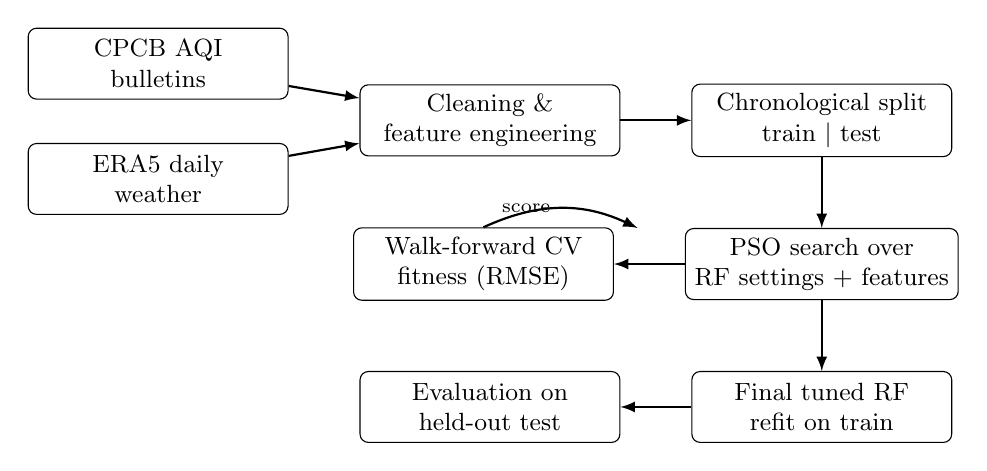
\begin{tikzpicture}[node distance=0.55cm, box/.style={draw, rounded corners=3pt, minimum width=3.3cm, minimum height=0.9cm, align=center, font=\small}, arr/.style={-latex, thick}]
\node[box] (a) {CPCB AQI\\bulletins};
\node[box, below=of a] (b) {ERA5 daily\\weather};
\node[box, right=0.9cm of a, yshift=-0.72cm] (c) {Cleaning \&\\feature engineering};
\node[box, right=0.9cm of c] (d) {Chronological split\\train $\mid$ test};
\node[box, below=0.9cm of d] (e) {PSO search over\\RF settings + features};
\node[box, left=0.9cm of e] (f) {Walk-forward CV\\fitness (RMSE)};
\node[box, below=0.9cm of e] (g) {Final tuned RF\\refit on train};
\node[box, left=0.9cm of g] (h) {Evaluation on\\held-out test};
\draw[arr] (a) -- (c); \draw[arr] (b) -- (c); \draw[arr] (c) -- (d);
\draw[arr] (d) -- (e); \draw[arr] (e.west) -- (f.east);
\draw[arr] (f.north) to[bend left=25] node[left,font=\scriptsize]{score} ([xshift=-0.6cm]e.north west);
\draw[arr] (e) -- (g); \draw[arr] (g) -- (h);
\end{tikzpicture}
\caption{System architecture of the PSO-optimized Random Forest pipeline}
\end{figure}

\subsection{Data Collection}

\topic{City Selection}
Delhi was selected because:
\begin{itemize}
\item It is the most polluted major city in the CPCB network, with strong seasonal swings
\item Its daily AQI record is long and nearly complete (26 missing days in 11.5 years)
\item Forecasts there have the largest public-health value
\end{itemize}

\topic{Data Sources and Period}
\begin{table}[H]
\centering
\caption{Data sources}
\begin{tabular}{|p{5.2cm}|p{5.6cm}|p{4.6cm}|}
\hline
\textbf{Source} & \textbf{Variables} & \textbf{Coverage} \\ \hline
CPCB daily AQI bulletins \cite{cpcb2014,urbanemissions} & City AQI, category, prominent pollutant & 1 May 2015 -- 25 Oct 2026; 4,170 reported days \\ \hline
ERA5 reanalysis via Open-Meteo \cite{hersbach2020,openmeteo} & Temperature, rain, humidity, wind, pressure, radiation, dew point & 1 Apr 2015 -- 25 Oct 2026; complete \\ \hline
\end{tabular}
\end{table}
The bulletin AQI is the official city value published by CPCB each day, averaged over Delhi's monitoring stations. The weather is taken at central Delhi (28.61\,N, 77.21\,E).

This period captures several distinct regimes:
\begin{itemize}
\item High-pollution years (2015--2019)
\item The COVID-19 lockdown and recovery (2020--2021)
\item Recent years under the National Clean Air Programme (2022--2026)
\end{itemize}

\topic{Data Validation}
The bulletin AQI was cross-checked against the independent Kaggle ``Air Quality Data in India (2015--2020)'' dataset over their 1,856 common days. The two series have a correlation of 0.927, which confirms that the bulletin values are consistent.

\subsection{Data Preprocessing}

\topic{Missing Value Treatment}
\begin{itemize}
\item AQI: 26 of 4,196 calendar days (0.6\%) have no bulletin
\item Weather: no missing values
\item Input features: forward fill, which uses only the last value known at prediction time
\item Target: never imputed; the 26 days with no observed AQI are removed as targets
\end{itemize}
Linear interpolation was avoided on purpose: it would use the next observation and leak future information into the features.

\topic{Normalization}
No scaling is applied to the Random Forest, because tree splits do not depend on feature scale. The linear and kernel baselines use standard scaling fitted on the training period only:
\begin{equation}
z = \frac{x - \mu_{train}}{\sigma_{train}}
\end{equation}

\subsection{Feature Engineering}
All features for day $t$ use only information available at the end of day $t$. A total of 32 features are created.

\lead{AQI History Features:}
\begin{itemize}
\item Current AQI and lags: $AQI_t, AQI_{t-1}, AQI_{t-2}, AQI_{t-3}, AQI_{t-7}$
\item Rolling means over 3, 7, 14 and 30 days
\item 7-day rolling standard deviation
\item Day-on-day change: $\Delta AQI_t = AQI_t - AQI_{t-1}$
\end{itemize}
\begin{equation}
\overline{AQI}_n(t) = \frac{1}{n}\sum_{i=0}^{n-1} AQI_{t-i}
\end{equation}

\lead{Weather Features:}
\begin{itemize}
\item Temperature (maximum, minimum, mean), dew point, relative humidity
\item Rainfall, and 3-day rainfall total
\item Wind speed (mean, maximum) and dominant wind direction
\item Surface pressure and shortwave radiation
\item Day-on-day change in minimum temperature, pressure, dew point and wind speed
\end{itemize}
Wind direction is circular, so it is encoded as sine and cosine:
\begin{equation}
(\sin\phi,\ \cos\phi), \qquad \phi = \text{direction in radians}
\end{equation}

\lead{Calendar Features:}
The day of year and day of week of the \emph{forecast} day are encoded cyclically:
\begin{equation}
doy_{sin} = \sin\!\left(\frac{2\pi\, d}{365.25}\right), \qquad doy_{cos} = \cos\!\left(\frac{2\pi\, d}{365.25}\right)
\end{equation}
This makes 31 December and 1 January neighbours.

\subsection{Random Forest Model Architecture}

\topic{Model Design}
\begin{itemize}
\item Input: 32 features for day $t$
\item Ensemble: $B$ regression trees (CART), each on a bootstrap sample
\item Split criterion: squared error
\item Output: the average of all tree predictions, the forecast AQI for day $t+1$
\end{itemize}

\topic{Why Random Forest}
\begin{itemize}
\item Captures non-linear effects and interactions between weather and pollution
\item Robust to correlated inputs such as lags and rolling means
\item Needs no feature scaling
\item Works well with about 3,000 training samples, where deep networks overfit easily
\item Provides feature importances for interpretation
\end{itemize}

\subsection{PSO Implementation}

\topic{Particle Representation}
Each particle is a 38-dimensional vector in the unit hypercube:
\begin{equation}
\mathbf{x} = [u_{trees}, u_{depth}, u_{split}, u_{leaf}, u_{features}, u_{samples}, u_{f_1}, \dots, u_{f_{32}}] \in [0,1]^{38}
\end{equation}
Implemented as a NumPy array. The hyperparameter part is decoded by:
\begin{verbatim}
def decode(position, space=SEARCH_SPACE):
    params = {}
    for u, p in zip(position, space):
        value = p.low + float(u) * (p.high - p.low)
        params[p.name] = int(round(value)) if p.integer \
                         else round(value, 3)
    return params
\end{verbatim}

The feature switches are decoded by:
\begin{verbatim}
def decode_solution(position, feature_names):
    params = decode(position[:6])
    switches = position[6:]
    keep = switches >= 0.5            # threshold transfer
    if keep.sum() < 3:                # never an empty model
        keep = np.zeros(len(switches), bool)
        keep[np.argsort(-switches)[:3]] = True
    return params, [f for f, k in zip(feature_names, keep) if k]
\end{verbatim}

\topic{Swarm Initialization}
A swarm of 12 particles is created with:
\begin{itemize}
\item Positions drawn uniformly from $[0,1]^{38}$, so each feature starts switched on with probability 0.5
\item Velocities drawn uniformly from $[-v_{max}, v_{max}]^{38}$
\item A seeded random number generator, so every run is reproducible
\end{itemize}

\topic{Fitness Evaluation}
The fitness of a particle is the mean RMSE over 5 expanding-window folds of the training period, using only the features the particle switches on:
\begin{equation}
F(\mathbf{x}) = \frac{1}{5}\sum_{k=1}^{5} RMSE\big(RF_{\theta(\mathbf{x})}\ \text{trained on folds } 1..k,\ \text{validated on fold } k+1\big)
\end{equation}
The model is always trained on earlier days and validated on later days. Identical decoded solutions (the same hyperparameters and the same feature subset) are cached, so the same configuration is never trained twice.

\topic{Velocity and Position Update}
\begin{verbatim}
def update_velocity(self, v, x, pbest, gbest, w):
    r1 = self.rng.random(x.shape)
    r2 = self.rng.random(x.shape)
    cognitive = self.cfg.c1 * r1 * (pbest - x)
    social = self.cfg.c2 * r2 * (gbest - x)
    return np.clip(w * v + cognitive + social,
                   -self.cfg.v_max, self.cfg.v_max)

def update_position(x, v):
    x_new = x + v
    for _ in range(2):          # reflect off the walls
        below, above = x_new < 0.0, x_new > 1.0
        x_new = np.where(below, -x_new, x_new)
        x_new = np.where(above, 2.0 - x_new, x_new)
        v = np.where(below | above, -v, v)
    return np.clip(x_new, 0.0, 1.0), v
\end{verbatim}

\topic{Best Updates}
After each evaluation:
\begin{equation}
\mathbf{p}_i \gets \mathbf{x}_i \ \text{ if } F(\mathbf{x}_i) < F(\mathbf{p}_i), \qquad \mathbf{g} \gets \arg\min_i F(\mathbf{p}_i)
\end{equation}

\topic{Termination Criteria}
The algorithm stops after 25 iterations, which gives $12 \times (25 + 1) = 312$ fitness evaluations per run.

\subsection{Training Procedure}

\topic{Data Splitting}
\begin{itemize}
\item Training: 3,115 days (30 May 2015 -- 31 December 2023), used for model fitting and all PSO tuning
\item Testing: 1,026 days (1 January 2024 -- 24 October 2026), used only for final evaluation
\end{itemize}
Temporal ordering is preserved, with no shuffling. The first 29 days are dropped because the 30-day rolling mean is incomplete.

\topic{Optimization Process}
For each of 5 independent PSO runs (seeds 0 to 4):
\begin{algorithmic}
\State Initialize the swarm
\For{each iteration}
  \State Decode every particle into RF hyperparameters
  \State Train RF on each walk-forward fold and record mean validation RMSE
  \State Update personal bests, global best, velocities and positions
\EndFor
\State Record the best configuration, its feature subset and its validation RMSE
\end{algorithmic}
The run with the lowest validation RMSE is selected; this rule was fixed before any test result was seen. Its hyperparameters and feature subset are refit on the full training period and evaluated once on the test period.

\subsection{Implementation Details}

\topic{Technology Stack}
\begin{itemize}
\item Python: 3.11
\item scikit-learn: 1.9 (Random Forest, metrics, baselines)
\item NumPy 2.4 and pandas 3.1: data handling and the PSO implementation
\item SciPy 1.17: statistical tests
\item Matplotlib 3.11: visualization
\item joblib: parallel execution of independent runs
\item pytest: automated tests
\end{itemize}

\topic{Computational Resources}
\begin{itemize}
\item CPU: Apple M5 Pro, 15 cores
\item RAM: 24 GB
\item GPU: not required
\end{itemize}

\topic{Reproducibility}
Ensured through:
\begin{itemize}
\item Fixed random seeds for PSO, random search and every forest
\item Configuration in a single file (\texttt{aqipso/config.py})
\item Version-pinned requirements
\item 16 automated tests, including checks that no feature uses future data and that the feature switches decode correctly
\end{itemize}

%================================================================ 0.6
\section{Experimental Setup and Test Functions}

\subsection{Experimental Configuration}

\topic{PSO Parameters}
\begin{table}[H]
\centering
\caption{PSO configuration parameters}
\begin{tabular}{|l|l|}
\hline
\textbf{Parameter} & \textbf{Value} \\ \hline
Swarm size & 12 particles \\
Number of iterations & 25 \\
Fitness evaluations per run & 312 \\
Inertia weight $w$ & 0.9 decreasing linearly to 0.4 \\
Cognitive coefficient $c_1$ & 1.5 \\
Social coefficient $c_2$ & 1.5 \\
Particle dimensions & 38 (6 hyperparameters + 32 feature switches) \\
Feature switch threshold & 0.5 (at least 3 features kept) \\
Velocity limit $v_{max}$ & 0.2 (per dimension) \\
Boundary handling & Reflection \\
Independent runs & 5 (seeds 0--4) \\ \hline
\end{tabular}
\end{table}

\topic{Random Forest Evaluation Parameters}
\begin{table}[H]
\centering
\caption{Model training and evaluation configuration}
\begin{tabular}{|l|l|}
\hline
\textbf{Parameter} & \textbf{Value} \\ \hline
Split criterion & Squared error \\
Fitness function & Mean RMSE over 5 walk-forward folds \\
Training period & 30 May 2015 -- 31 Dec 2023 (3,115 days) \\
Test period & 1 Jan 2024 -- 24 Oct 2026 (1,026 days) \\
Forest random seed & 42 (search); 100--109 (robustness check) \\ \hline
\end{tabular}
\end{table}

\topic{Hyperparameter Search Space}
The search space is shown in Table 2 (Section 0.4.2). It covers forests from 50 to 300 trees, depths from 3 to 30, and feature and sample fractions from very small to complete.

\subsection{Baseline Models}
To validate the effectiveness of PSO optimization, we compare against:

\topic{Baseline 1: Persistence}
Tomorrow's AQI is predicted to equal today's ($\hat{y}_{t+1} = y_t$). This is the minimum any useful model must beat.

\topic{Baseline 2: Default Random Forest}
A Random Forest with scikit-learn's default hyperparameters:
\begin{itemize}
\item Trees: 100
\item Maximum depth: unlimited
\item Minimum samples to split: 2; minimum samples per leaf: 1
\item Features per split: all (1.0); bootstrap sample: all days
\end{itemize}

\topic{Baseline 3: Random Search}
Random selection as a control for PSO:
\begin{itemize}
\item 312 random points in the same 38-dimensional space, the same budget as PSO
\item Same decoding, same feature switches and same fitness function
\item 5 independent runs; best configuration selected
\end{itemize}

\topic{Ablation: Hyperparameter-Only Search}
To measure what feature selection adds, PSO and random search were also run over the 6 hyperparameters alone, with all 32 features always used (5 runs each, same budget). The best hyperparameter-only PSO model is also evaluated on the test period.

\topic{Baseline 4: Traditional Models}
Untuned models trained on the same 32 features:
\begin{itemize}
\item Ridge regression ($\alpha = 1$, standardized inputs)
\item Support Vector Regression (RBF kernel, $C = 100$, $\epsilon = 5$)
\item Gradient Boosting Regressor (default settings)
\end{itemize}

\subsection{Test Functions and Benchmarks}

\topic{Optimization Test Functions}
To validate the PSO implementation, it was first tested on standard benchmarks in 6 dimensions (30 particles, 200 iterations, 5 seeds).

\lead{Sphere Function:}
\begin{equation}
f(\mathbf{x}) = \sum_{i=1}^{n} x_i^2, \qquad x_i \in [-100, 100]
\end{equation}
Global minimum: $f(0,\dots,0) = 0$. Unimodal; tests convergence speed.

\lead{Rastrigin Function:}
\begin{equation}
f(\mathbf{x}) = 10n + \sum_{i=1}^{n}\left[x_i^2 - 10\cos(2\pi x_i)\right], \qquad x_i \in [-5.12, 5.12]
\end{equation}
Highly multi-modal; tests escape from local minima.

\lead{Rosenbrock Function:}
\begin{equation}
f(\mathbf{x}) = \sum_{i=1}^{n-1}\left[100(x_{i+1} - x_i^2)^2 + (1 - x_i)^2\right], \qquad x_i \in [-5, 5]
\end{equation}
Tests convergence along a narrow curved valley.

\begin{table}[H]
\centering
\caption{PSO results on benchmark functions (6 dimensions, 5 runs; global minimum 0)}
\begin{tabular}{|l|c|c|c|}
\hline
\textbf{Function} & \textbf{Mean best $f$} & \textbf{Std Dev} & \textbf{Best run} \\ \hline
Sphere & $1.9\times10^{-17}$ & $3.2\times10^{-17}$ & $1.0\times10^{-18}$ \\
Rastrigin & 2.99 & 1.41 & 1.99 \\
Rosenbrock & 1.10 & 0.19 & 0.84 \\ \hline
\end{tabular}
\end{table}

PSO solves the Sphere function to machine precision, which confirms that the operators are implemented correctly. On Rastrigin it reaches low values but stops in a local minimum near $f \approx 2$, with two coordinates trapped in the neighbouring wells at $\pm 1$. On Rosenbrock it reaches the valley quickly but advances slowly along it. These are the expected strengths and weaknesses of global-best PSO.

\begin{figure}[H]
\centering
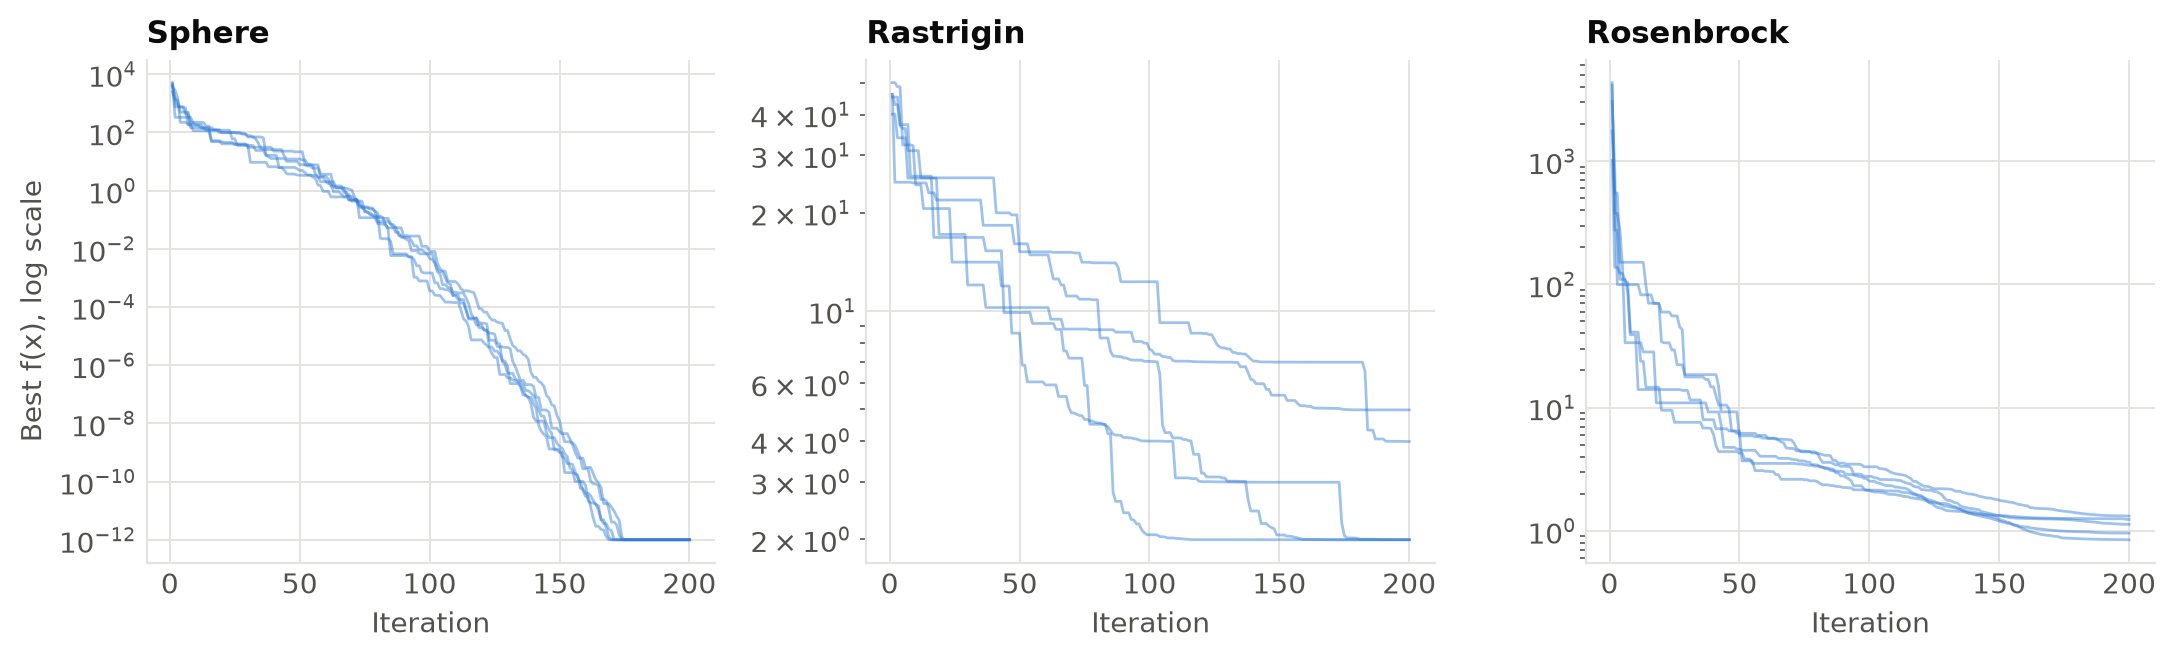
\includegraphics[width=\textwidth]{figures/16_benchmark_convergence.png}
\caption{PSO convergence on the three benchmark functions (5 runs each, log scale)}
\end{figure}

\subsection{Cross-Validation Strategy}

\topic{Time Series Cross-Validation}
For PSO fitness evaluation, walk-forward validation with an expanding window is used:
\begin{itemize}
\item 5 temporal folds over the training period
\item Each fold trains on all earlier days and validates on the next block of 519 days
\item The first fold trains on 520 days; the last trains on 2,596 days
\item Fitness = average RMSE across the 5 folds
\end{itemize}
Shuffled $k$-fold cross-validation was not used, because it would let the model train on days after the ones it is validated on.

\topic{Hold-Out Test}
The test period (2024 to 2026) is never used during the search. It is used once, to evaluate the final selected model.

\subsection{Sensitivity Analysis}

\topic{PSO Parameter Sensitivity}
The effect of PSO's own parameters was tested on the 6-dimensional Rastrigin function, with 100 iterations and 10 seeds per variant:

\begin{table}[H]
\centering
\caption{PSO parameter sensitivity on Rastrigin (lower is better)}
\begin{tabular}{|l|c|c|c|}
\hline
\textbf{Variant} & \textbf{Mean best} & \textbf{Std Dev} & \textbf{Best run} \\ \hline
Base: 20 particles, $w$ 0.9$\to$0.4, $c_1 = c_2 = 1.5$ & 6.63 & 2.61 & 2.99 \\
10 particles & 5.40 & 2.78 & 1.04 \\
40 particles & 3.59 & 2.11 & 1.00 \\
Constant inertia $w = 0.7$ & 3.73 & 1.84 & 1.99 \\
Constant inertia $w = 0.4$ & 5.27 & 2.57 & 1.00 \\
$c_1 = 2.0$, $c_2 = 1.0$ (more cognitive) & 4.77 & 3.42 & 1.00 \\
$c_1 = 1.0$, $c_2 = 2.0$ (more social) & 3.76 & 2.39 & 1.03 \\ \hline
\end{tabular}
\end{table}

Results show high run-to-run variance on this multi-modal function: standard deviations are 2 to 3 points, so differences of 1 to 2 points between variants are within noise. A larger swarm (40 particles) gave the lowest mean, as expected from its broader exploration. With only 100 iterations, the decreasing-inertia schedule spends much of the run exploring and did not beat constant $w = 0.7$; with the 25-iteration budget of the main experiment, the choice of schedule matters less than the swarm's ability to locate the right region.

\subsection{Statistical Significance Testing}

\topic{Block Bootstrap}
Daily forecast errors are autocorrelated, so ordinary resampling would overstate confidence. A moving-block bootstrap \cite{kunsch1989} resamples whole weeks (block length 7, 5,000 resamples) and computes the RMSE gain:
\begin{equation}
\Delta = RMSE_{baseline} - RMSE_{tuned}
\end{equation}
The 2.5th and 97.5th percentiles of $\Delta$ give a 95\% confidence interval.

\topic{Paired t-test}
Compares the daily squared errors of the default and tuned models:
\begin{equation}
t = \frac{\bar{d}}{s_d / \sqrt{n}}
\end{equation}
where $\bar{d}$ is the mean difference and $s_d$ the standard deviation of differences.

\topic{Wilcoxon Signed-Rank Test}
A non-parametric alternative for non-normal differences:
\begin{equation}
W = \sum_{i=1}^{n} \operatorname{sgn}(x_{2,i} - x_{1,i}) \cdot R_i
\end{equation}

\subsection{Computational Efficiency Metrics}

\topic{Training Time Analysis}
Measured for each approach:
\begin{itemize}
\item Wall-clock time per search run
\item Number of fitness evaluations, and how many were unique after caching
\item Iteration at which the global best stopped improving
\end{itemize}
The 20 search runs (PSO and random search, each with and without feature selection, 5 seeds each) were executed in parallel on 15 CPU cores.

%================================================================ 0.7
\section{Results and Discussion}

\subsection{PSO Convergence Analysis}

\topic{Fitness Evolution}
Figure 3 shows the global-best validation RMSE across iterations for all five PSO runs of the joint (hyperparameter and feature) search:
\begin{itemize}
\item Iteration 1: mean global best = 41.22 (already below the default forest's 41.52)
\item Iteration 10: mean global best = 40.20
\item Iteration 25: mean global best = 39.94; best run = 39.73
\end{itemize}
The joint search keeps improving for longer than a hyperparameter-only search, because there are many more feature subsets to explore. The global best was still improving at iterations 22 to 25 in every run, so a larger budget would probably lower the validation error further.

\begin{figure}[H]
\centering
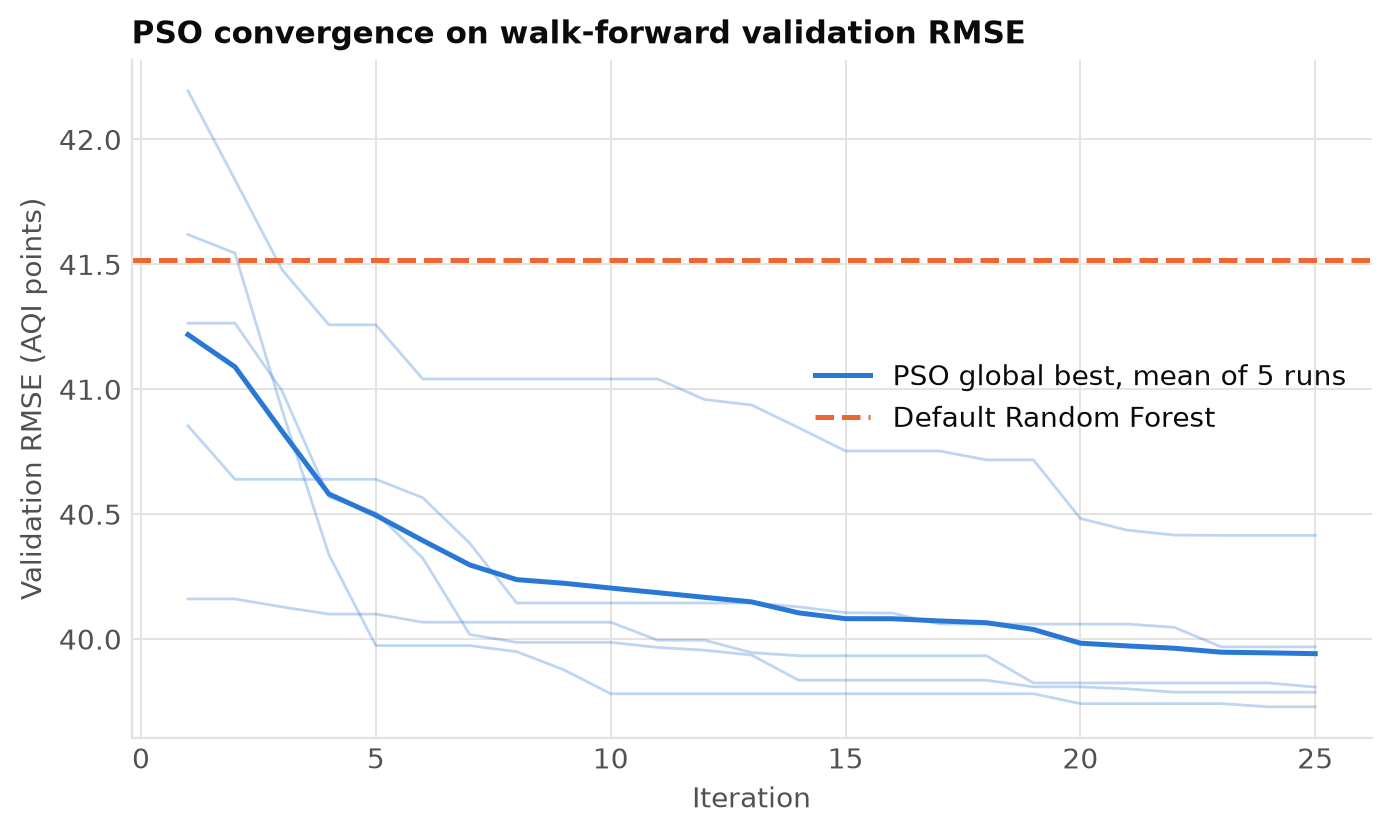
\includegraphics[width=0.88\textwidth]{figures/04_pso_convergence.png}
\caption{PSO convergence on walk-forward validation RMSE (5 runs)}
\end{figure}

\topic{Swarm Diversity}
Diversity is measured as the mean distance of particles from the swarm centre:
\begin{equation}
D_k = \frac{1}{N}\sum_{i=1}^{N}\left\lVert \mathbf{x}_i^k - \bar{\mathbf{x}}^k \right\rVert
\end{equation}
In the selected run, diversity fell from 1.28 to 0.19 while the swarm's mean RMSE fell from 42.97 to 39.85, showing the expected shift from exploration to exploitation as the inertia weight decreased. Diversity is larger than in a 6-dimensional search simply because distances are measured in 38 dimensions.

\begin{figure}[H]
\centering
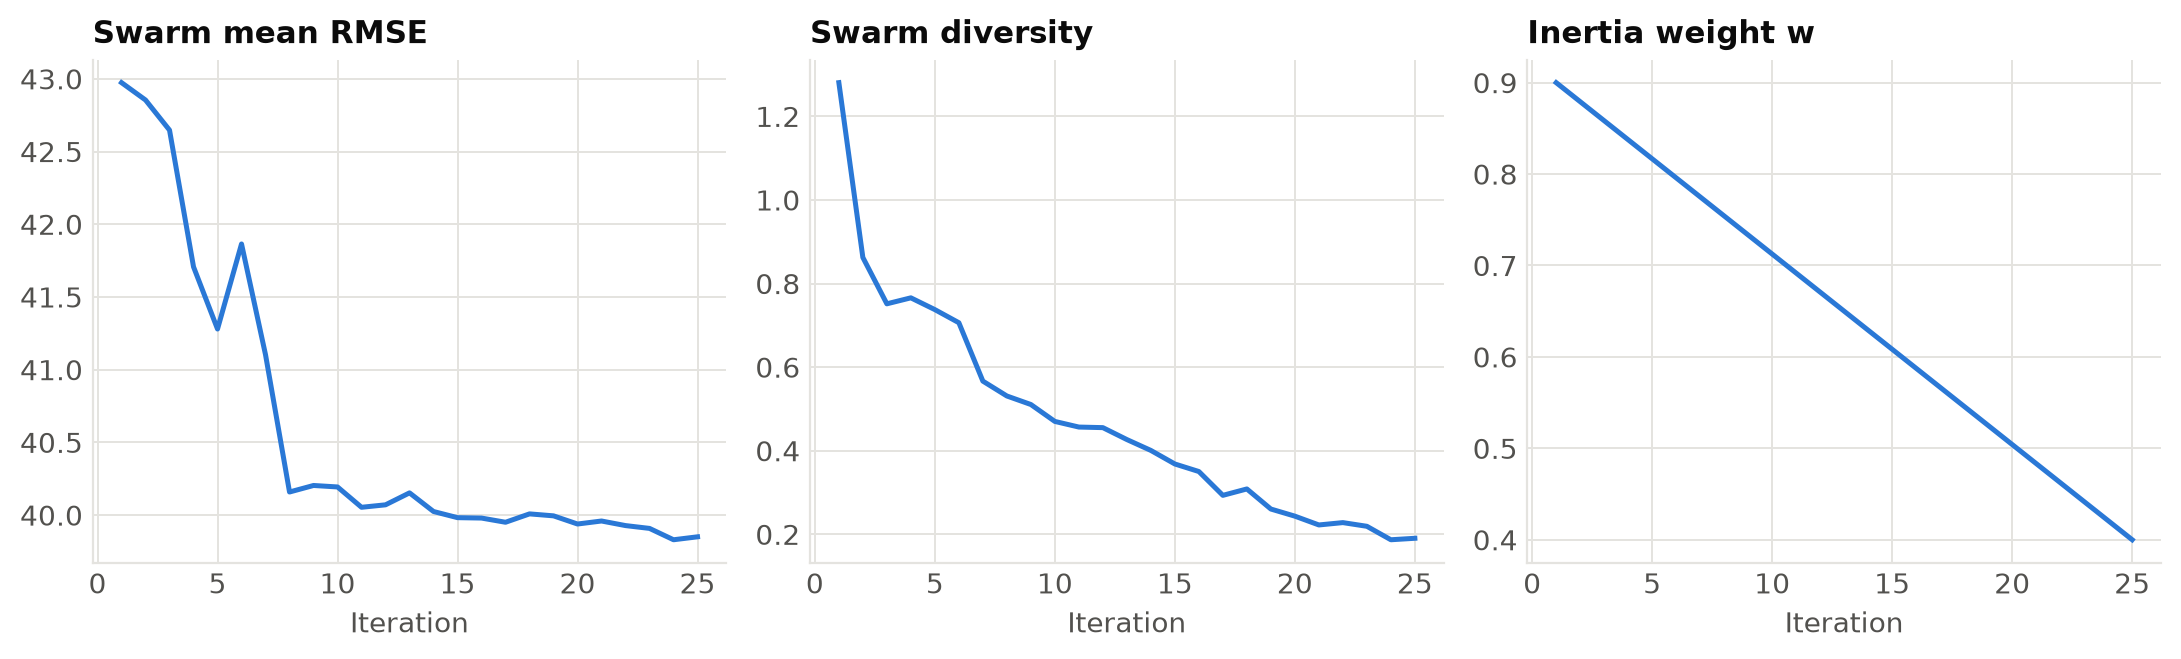
\includegraphics[width=\textwidth]{figures/06_swarm_dynamics.png}
\caption{Swarm mean fitness, diversity and inertia weight in the selected run}
\end{figure}

\subsection{Optimal Configuration}
The run with the lowest validation RMSE (seed 0, RMSE 39.73) was selected.

\begin{table}[H]
\centering
\caption{Best configuration found by PSO}
\begin{tabular}{|l|c|c|c|}
\hline
\textbf{Setting} & \textbf{Default} & \textbf{PSO, hyperparameters only} & \textbf{PSO, joint (final)} \\ \hline
n\_estimators & 100 & 291 & 224 \\
max\_depth & Unlimited & 17 & 18 \\
min\_samples\_split & 2 & 6 & 8 \\
min\_samples\_leaf & 1 & 3 & 2 \\
max\_features & 1.0 & 0.797 & 0.799 \\
max\_samples & 1.0 & 0.655 & 0.592 \\
Features used & 32 & 32 & 14 \\
Validation RMSE & 41.52 & 40.66 & \textbf{39.73} \\ \hline
\end{tabular}
\end{table}

\lead{Key Insights:}
\begin{itemize}
\item Both searches found very similar hyperparameters: depth near 17, about 80\% of features tried per split, and 60 to 65\% of days per tree
\item Limited depth and leaves of 2 to 3 days regularize each tree; feature and sample sub-sampling decorrelate the trees
\item Feature selection removed 18 of 32 features and lowered validation RMSE by a further 0.93 points
\end{itemize}

\begin{figure}[H]
\centering
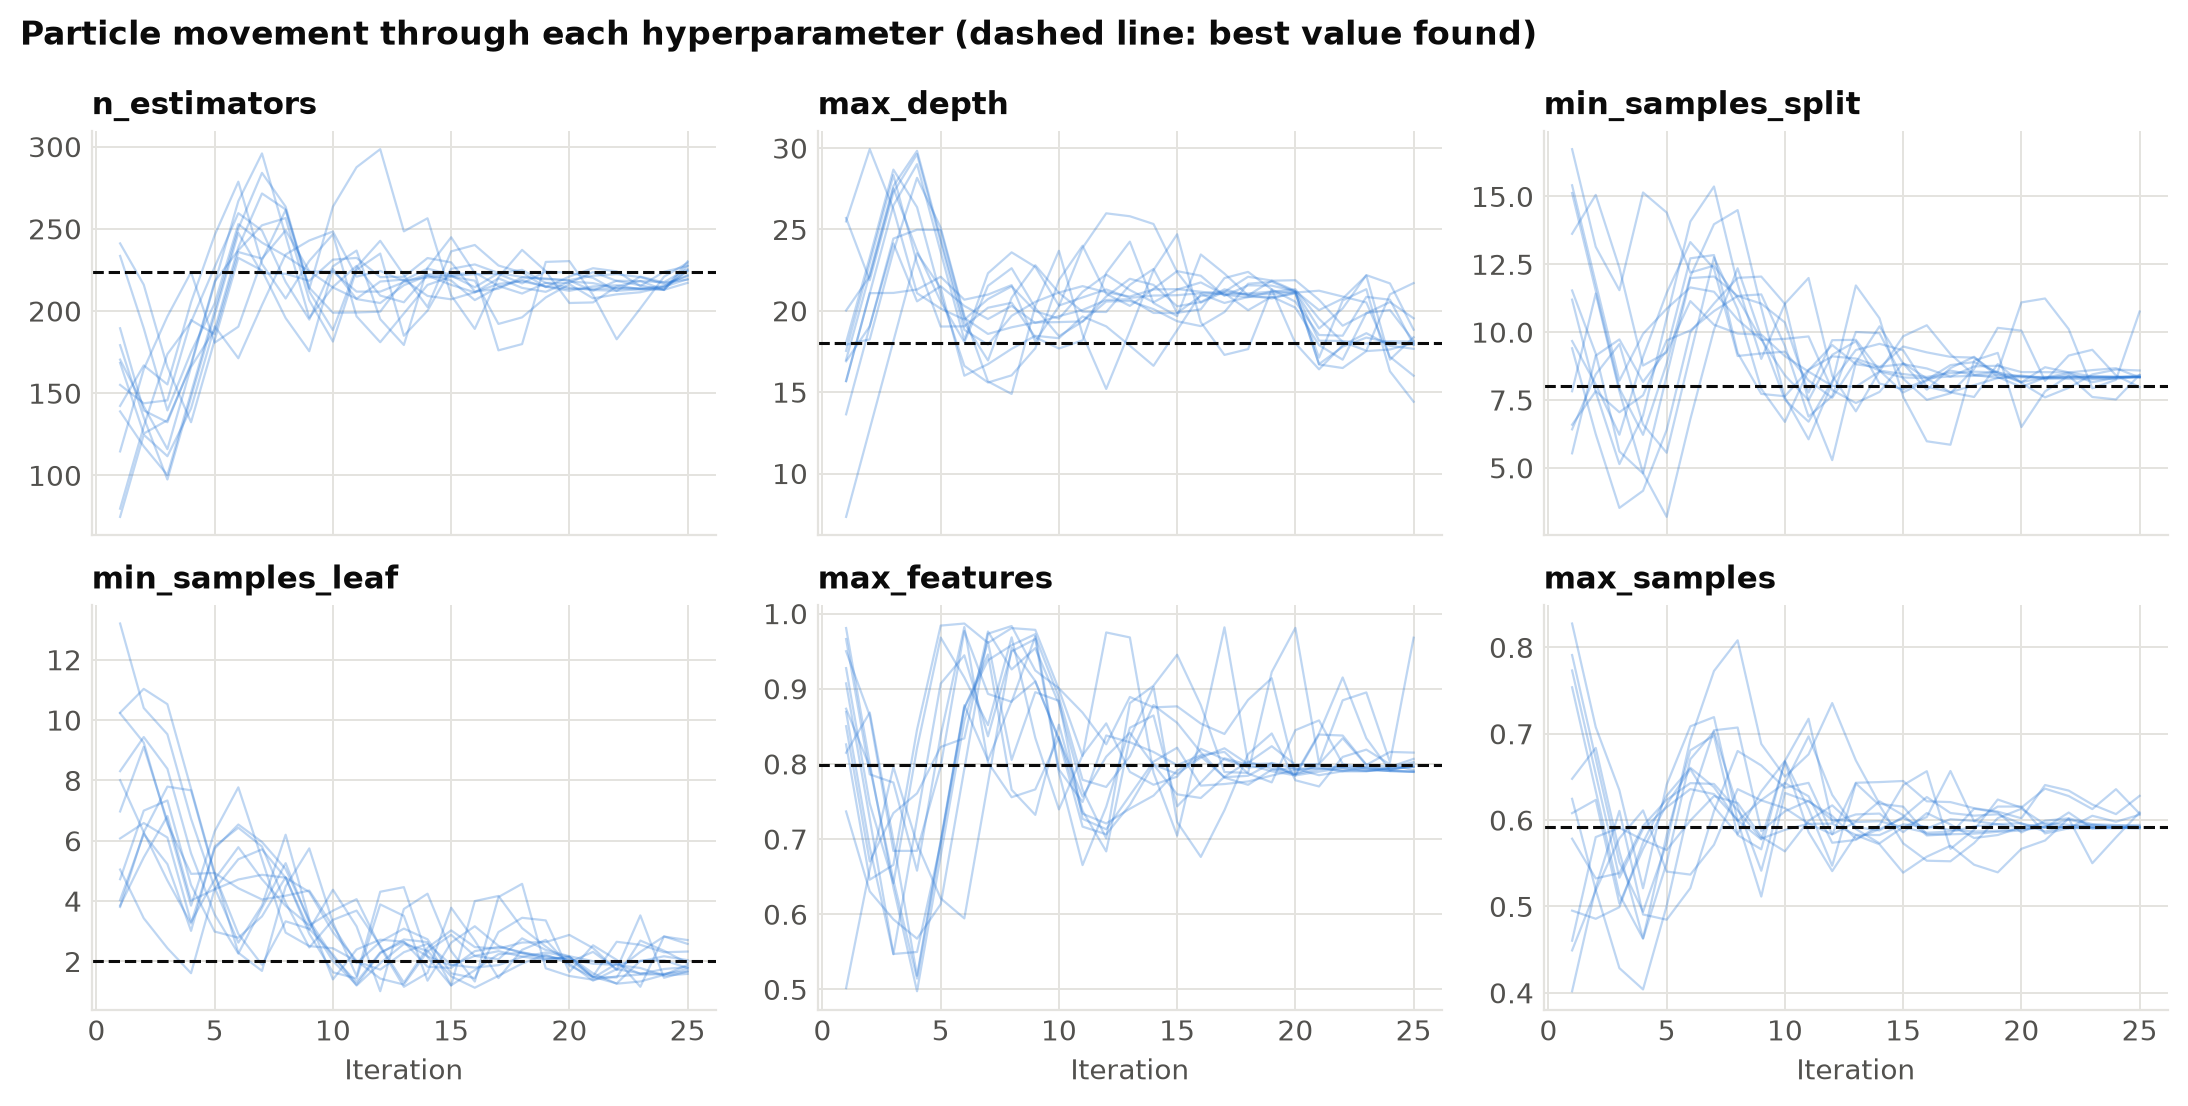
\includegraphics[width=\textwidth]{figures/07_parameter_paths.png}
\caption{Particle trajectories through each hyperparameter in the selected run}
\end{figure}

\subsection{Feature Selection Results}
The 14 features kept by the final model are: today's AQI, yesterday's AQI, the 3-day and 30-day mean AQI, the day-on-day AQI change, maximum temperature, rainfall, 3-day rainfall, maximum wind speed, the change in mean wind speed, wind direction (sine and cosine), shortwave radiation, and one day-of-week term.

\lead{Consistent choices across the five runs:}
\begin{itemize}
\item \textbf{Always kept (5 of 5 runs):} today's AQI, 3-day rainfall, shortwave radiation, wind direction (sine), change in mean wind speed, day of week (cosine)
\item \textbf{Never kept (0 of 5 runs):} relative humidity, surface pressure, dew point, and the AQI two days ago
\item The runs kept between 12 and 18 features
\end{itemize}
The kept variables are those that physically control pollution: wind and its changes disperse it, rain washes it out, and solar radiation drives the daytime mixing layer. Humidity, pressure and dew point are strongly correlated with temperature and season, so they add little once those are present. Recent AQI is represented by today's value and short averages, which makes the separate lags redundant.

\begin{figure}[H]
\centering
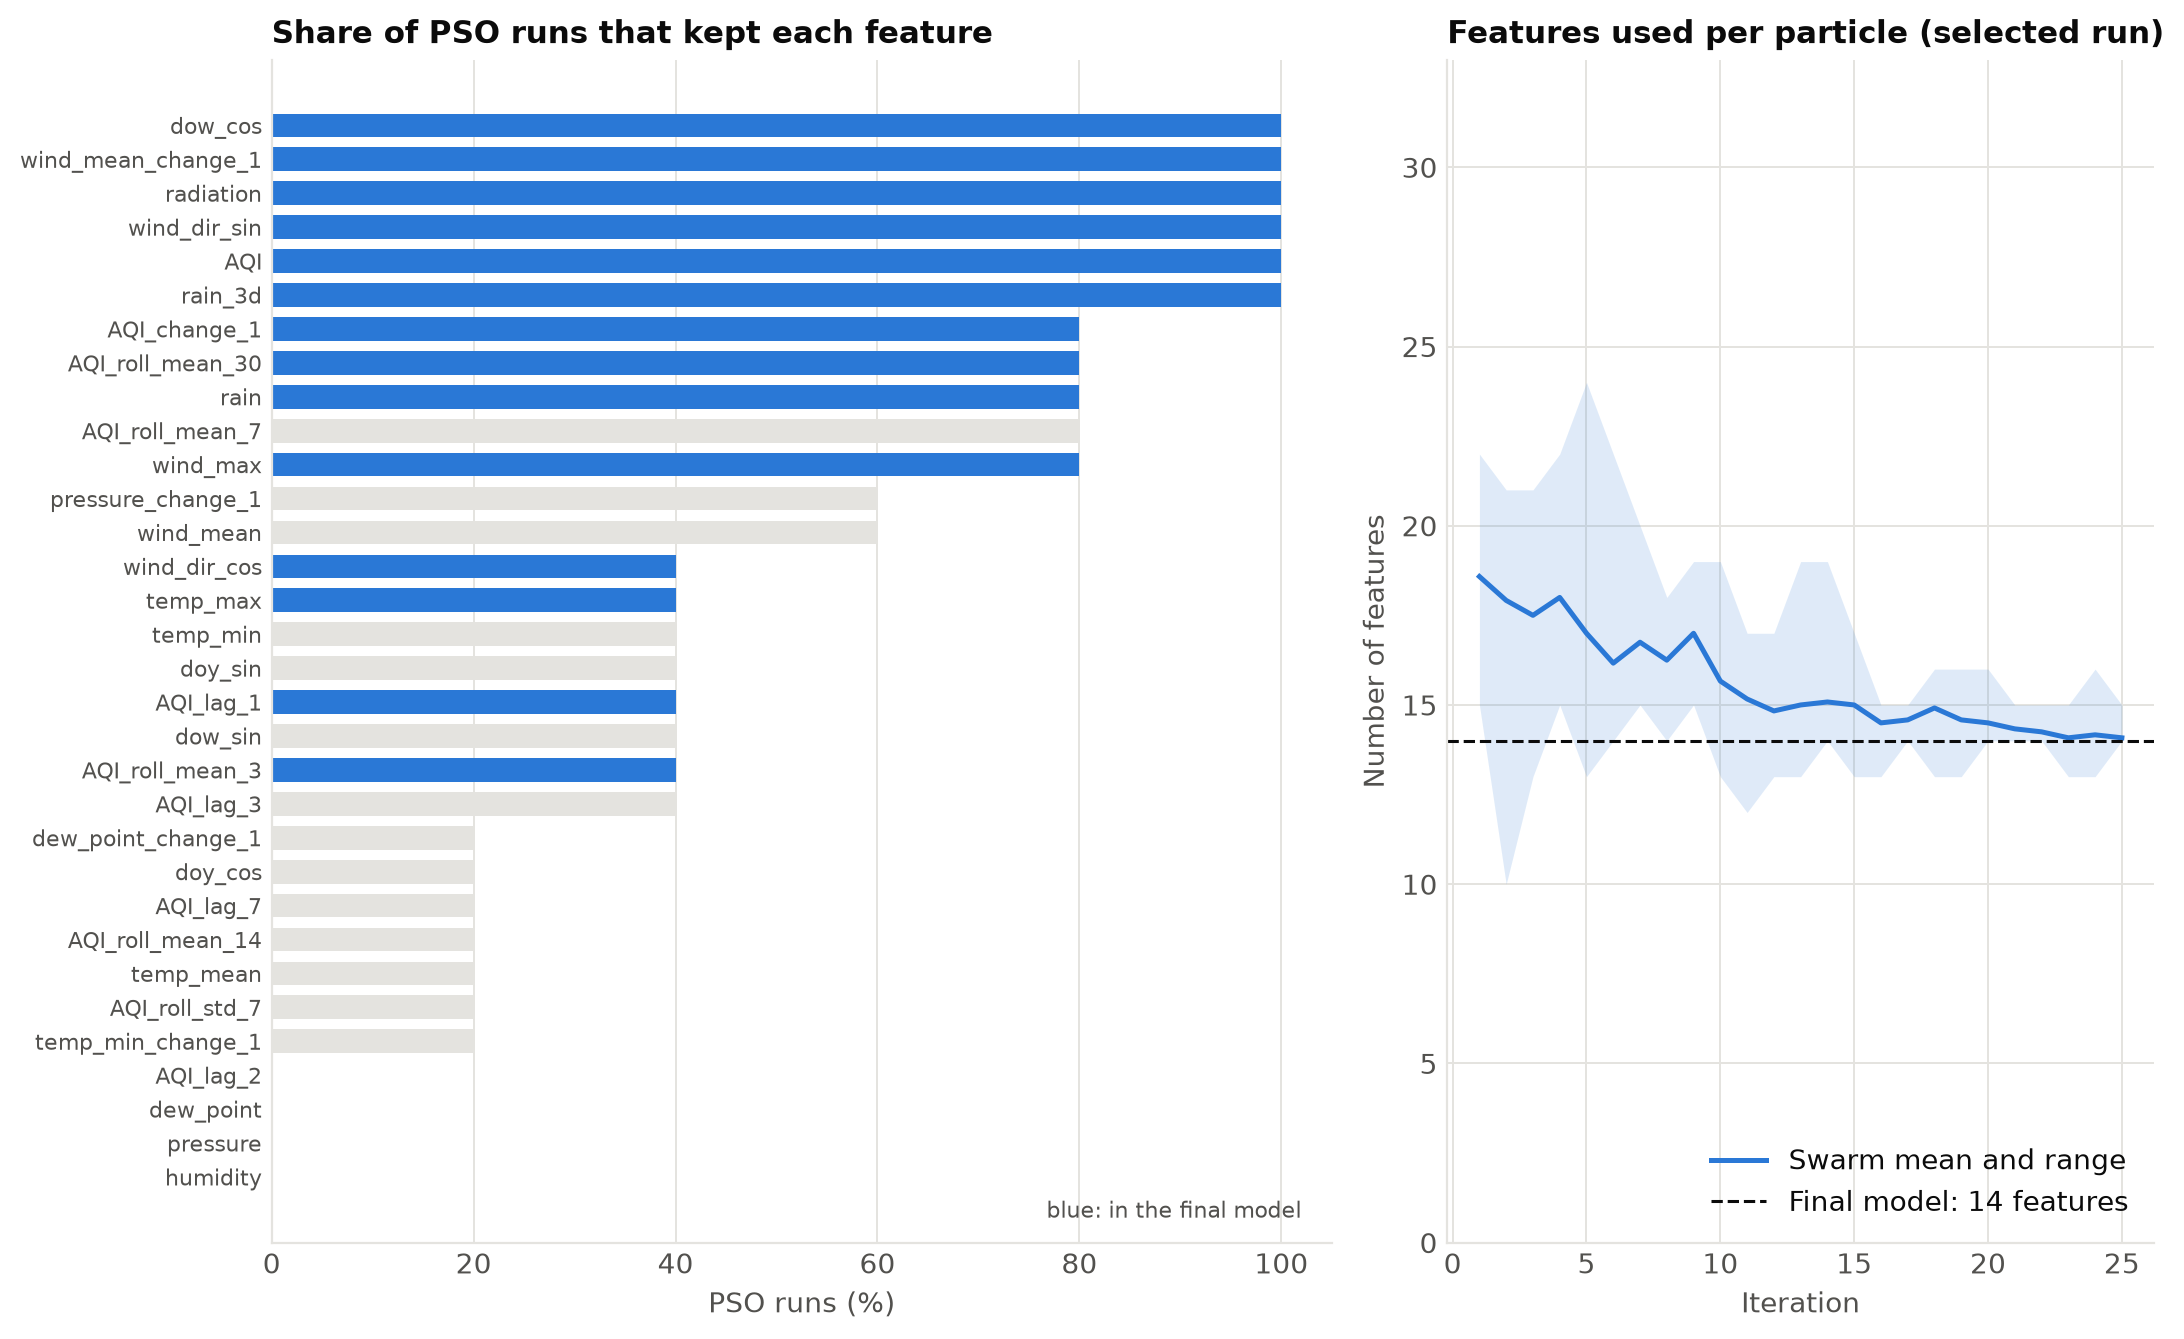
\includegraphics[width=\textwidth]{figures/17_feature_selection.png}
\caption{Share of PSO runs that kept each feature (left) and the number of features used by the swarm in the selected run (right)}
\end{figure}

\subsection{Prediction Performance}

\topic{Test Period Results}
\begin{table}[H]
\centering
\small\setlength{\tabcolsep}{4pt}
\caption{Test performance, 1 Jan 2024 -- 24 Oct 2026 (1,026 days)}
\begin{tabular}{|l|c|c|c|c|}
\hline
\textbf{Metric} & \textbf{Persistence} & \textbf{Default RF} & \textbf{PSO, hyp. only} & \textbf{PSO, joint (final)} \\ \hline
RMSE & 40.21 & 33.85 & \textbf{33.57} & 33.77 \\
MAE & 28.97 & 25.38 & \textbf{25.14} & 25.15 \\
Median absolute error & 21.00 & 19.39 & 18.87 & \textbf{18.08} \\
MAPE (\%) & 17.16 & 15.89 & 15.74 & \textbf{15.65} \\
$R^2$ & 0.832 & 0.881 & \textbf{0.883} & 0.882 \\
Category accuracy & 0.688 & \textbf{0.719} & 0.715 & 0.714 \\
Category precision (macro) & 0.547 & 0.607 & 0.611 & \textbf{0.622} \\
Category recall (macro) & 0.548 & \textbf{0.555} & 0.552 & 0.552 \\
Category F1 (macro) & 0.548 & 0.568 & 0.566 & \textbf{0.569} \\
AUC, AQI $>$ 300 & 0.978 & 0.986 & \textbf{0.987} & 0.986 \\ \hline
\end{tabular}
\end{table}

\lead{Analysis:}
\begin{itemize}
\item The final model beats the default forest on RMSE, MAE, median error, MAPE, $R^2$, category precision and F1, but by small margins (RMSE 0.25\%, median error 6.8\%)
\item It is slightly worse than the hyperparameter-only PSO model on RMSE (33.77 against 33.57), even though its validation error was much lower
\item All forests beat persistence substantially (RMSE 16.0\% lower for the final model)
\item All forests detect \emph{Very Poor} or worse days very well (AUC 0.986 to 0.987)
\end{itemize}

\begin{figure}[H]
\centering
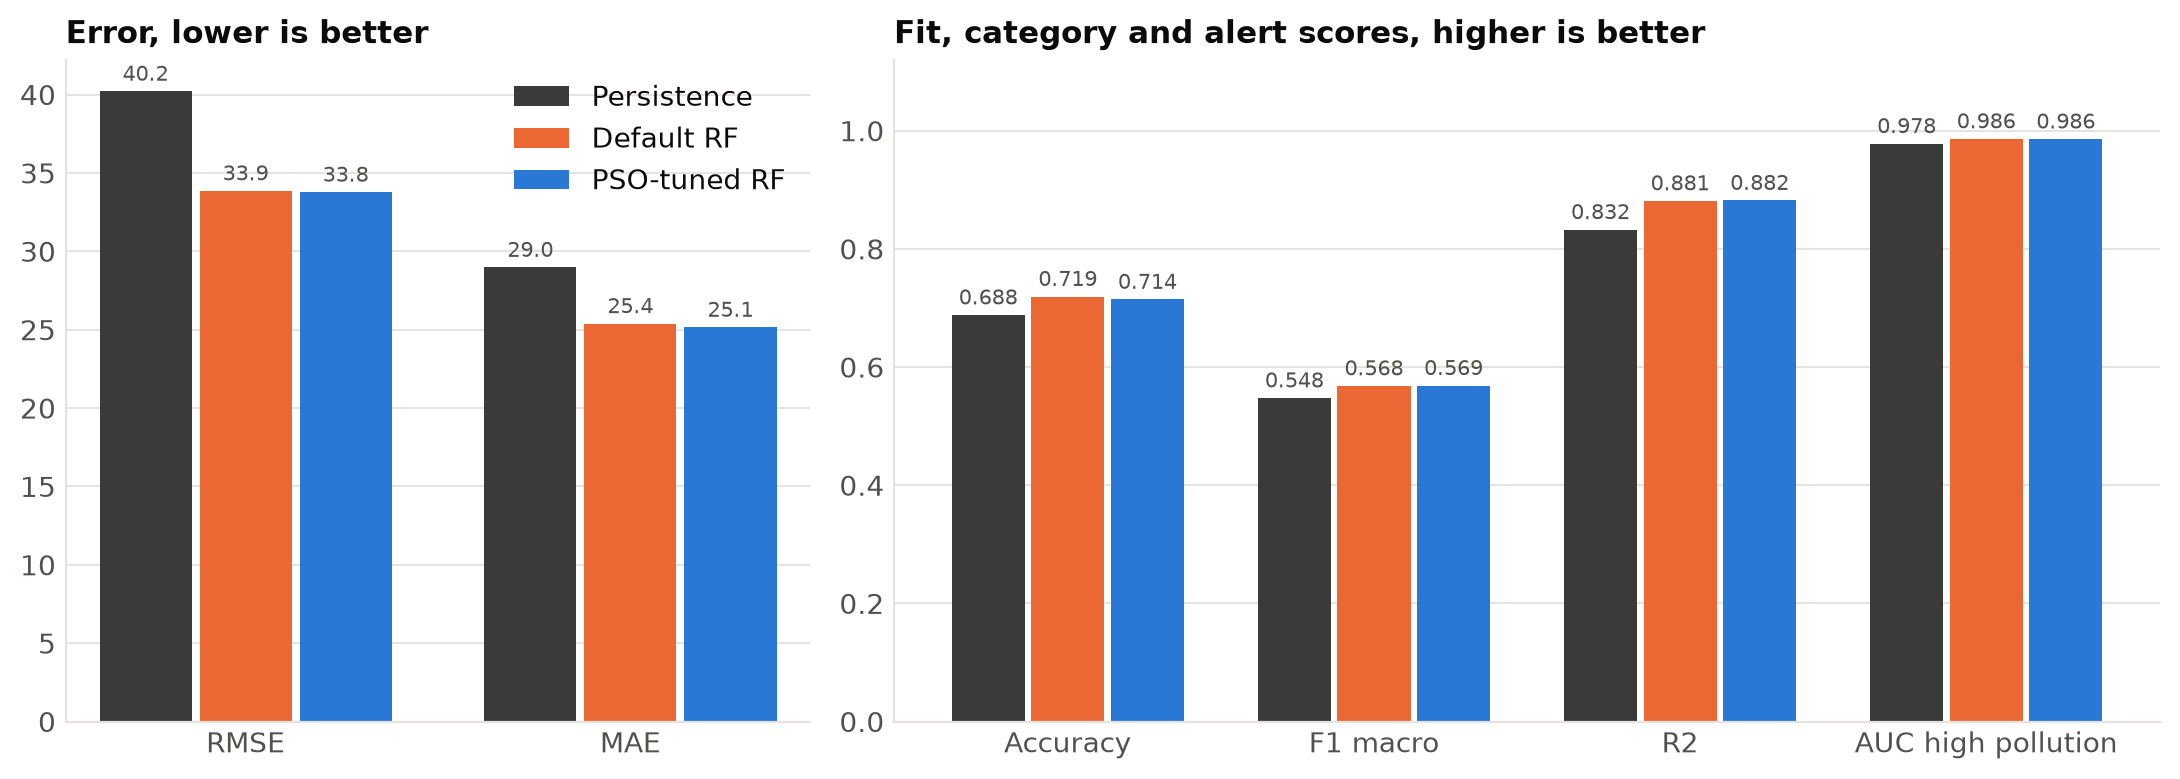
\includegraphics[width=\textwidth]{figures/08_metric_comparison.png}
\caption{Test metrics of persistence, the default forest and the final PSO model}
\end{figure}

\subsection{Temporal Performance Analysis}

\topic{Performance Across Years and Seasons}
\begin{table}[H]
\centering
\small\setlength{\tabcolsep}{4pt}
\caption{Test RMSE by period}
\begin{tabular}{|l|c|c|c|c|c|c|}
\hline
\textbf{Period} & \textbf{Days} & \textbf{Mean AQI} & \textbf{Persist.} & \textbf{Default RF} & \textbf{PSO hyp.} & \textbf{PSO joint} \\ \hline
2024 & 365 & 208.6 & 41.98 & \textbf{34.12} & 34.20 & 34.30 \\
2025 & 365 & 201.0 & 38.38 & 34.23 & \textbf{33.66} & 34.07 \\
2026 (to 24 Oct) & 296 & 166.6 & 40.17 & 33.04 & \textbf{32.67} & 32.72 \\
Winter (Oct--Feb) & 385 & 281.6 & 48.29 & 40.22 & \textbf{40.16} & 40.22 \\
Rest of year (Mar--Sep) & 641 & 141.0 & 34.45 & 29.37 & \textbf{28.90} & 29.21 \\ \hline
\end{tabular}
\end{table}

Errors are largest in the winter smog season, when AQI is highest and most volatile. In every period the three forests are within 0.6 points of each other, while persistence is 4 to 8 points worse.

\begin{figure}[H]
\centering
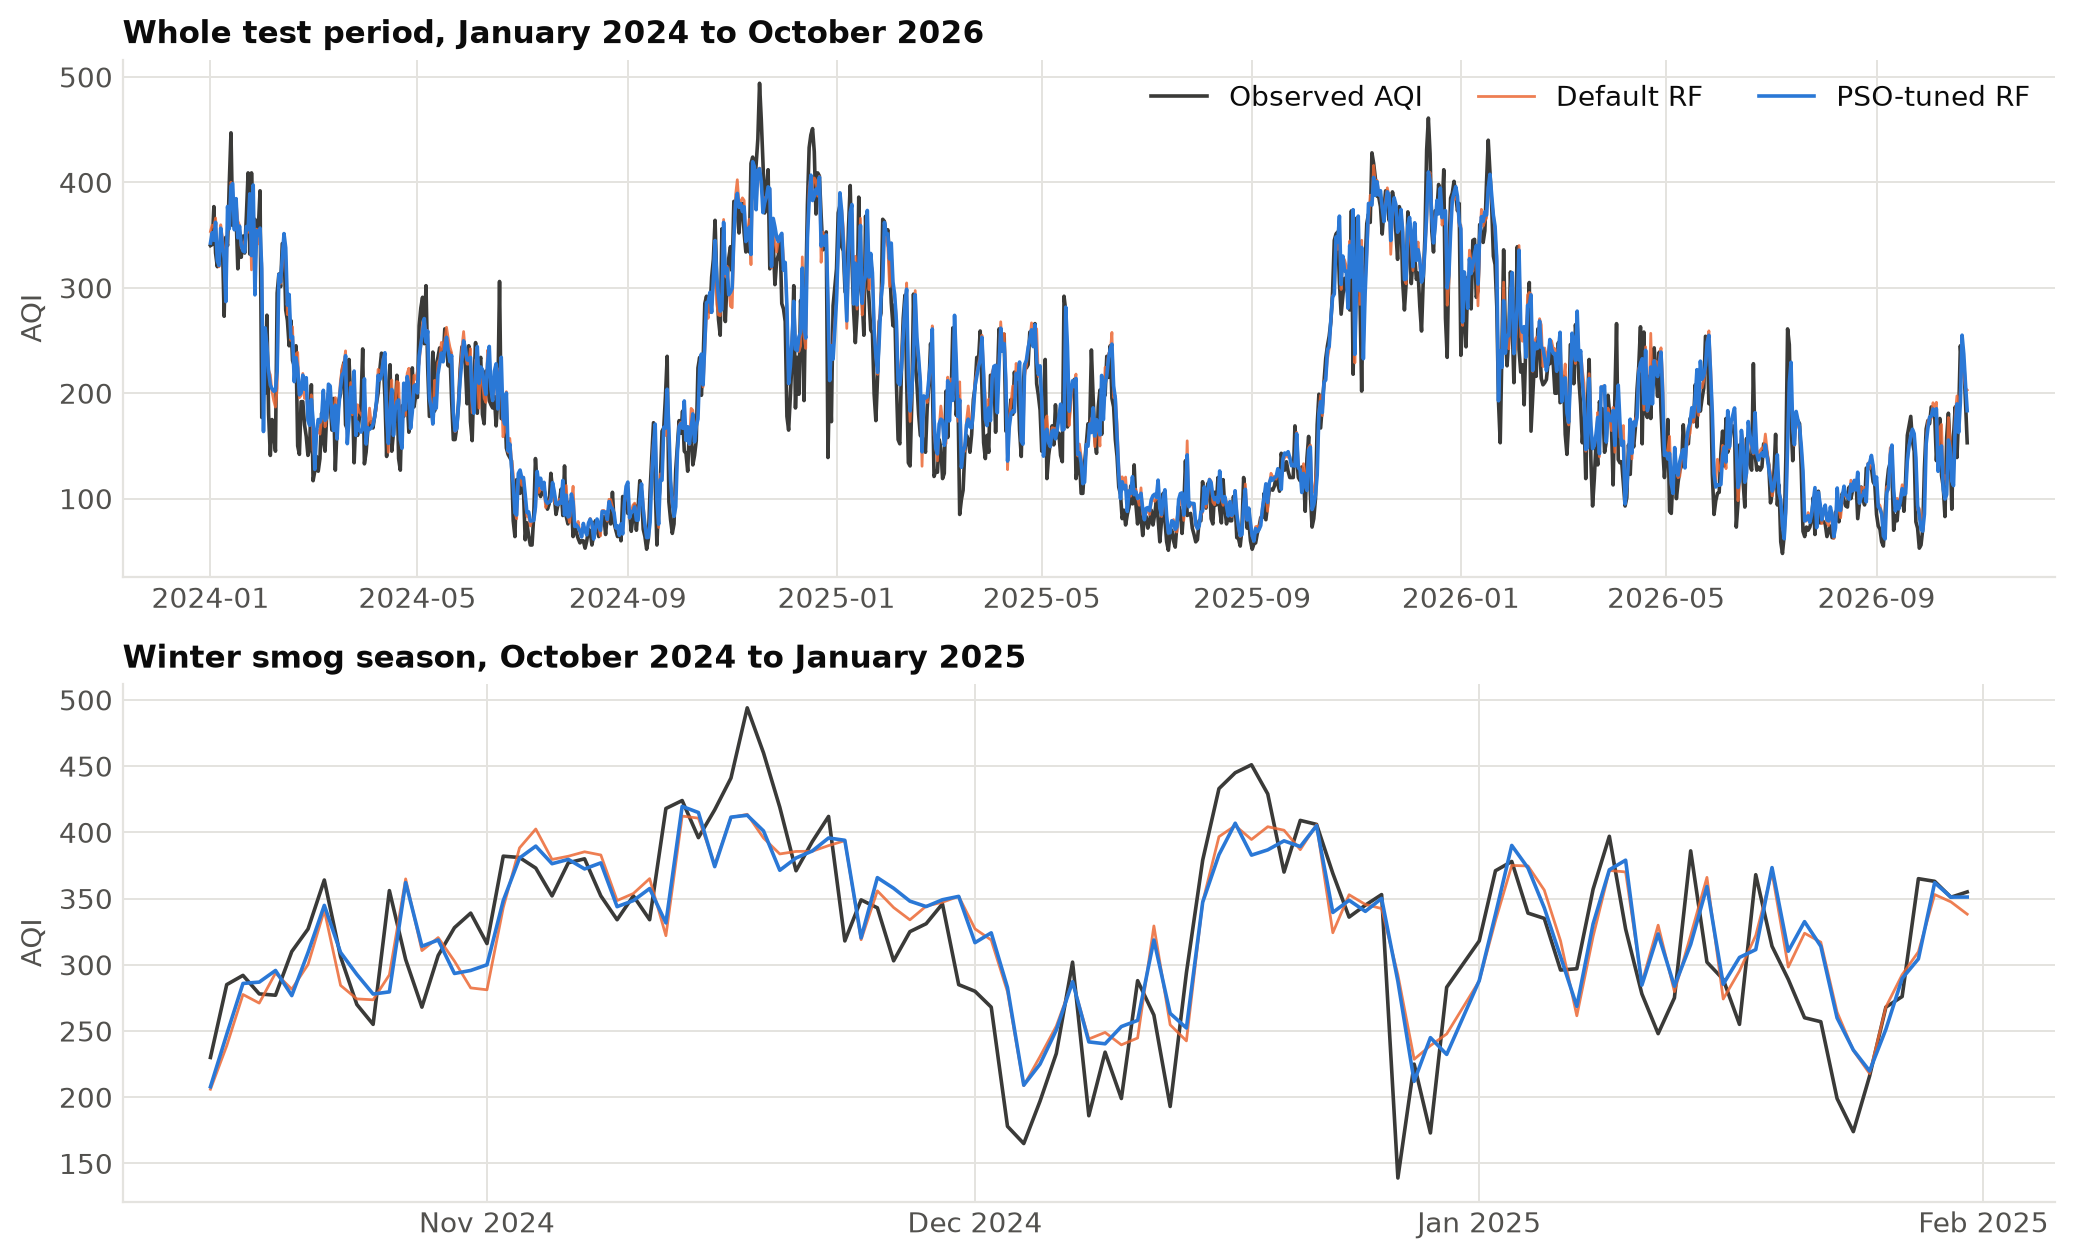
\includegraphics[width=\textwidth]{figures/09_forecast_timeline.png}
\caption{Observed and forecast AQI over the test period, with the 2024--25 winter in detail}
\end{figure}

\subsection{Comparison with Baseline Models}

\topic{Performance Comparison}
\begin{table}[H]
\centering
\caption{Model comparison on the test period}
\begin{tabular}{|l|c|c|c|}
\hline
\textbf{Model} & \textbf{RMSE} & \textbf{MAE} & \textbf{$R^2$} \\ \hline
Persistence & 40.21 & 28.97 & 0.832 \\
Default Random Forest & 33.85 & 25.38 & 0.881 \\
\textbf{PSO Random Forest, joint (final)} & \textbf{33.77} & \textbf{25.15} & \textbf{0.882} \\
Gradient Boosting (default) & 33.61 & 25.33 & 0.883 \\
PSO Random Forest, hyperparameters only & 33.57 & 25.14 & 0.883 \\
Support Vector Regression & 33.46 & 25.40 & 0.884 \\
Ridge regression & 33.45 & 25.27 & 0.884 \\ \hline
\end{tabular}
\end{table}

\lead{Key Findings:}
\begin{itemize}
\item All learned models fall within 0.4 RMSE points of each other and beat persistence by 16 to 17\%
\item Ridge regression and SVR have the lowest RMSE. With good lag and weather features, next-day AQI is close to a linear problem
\item The final PSO model uses less than half the features of every other model at very similar accuracy
\end{itemize}

\begin{figure}[H]
\centering
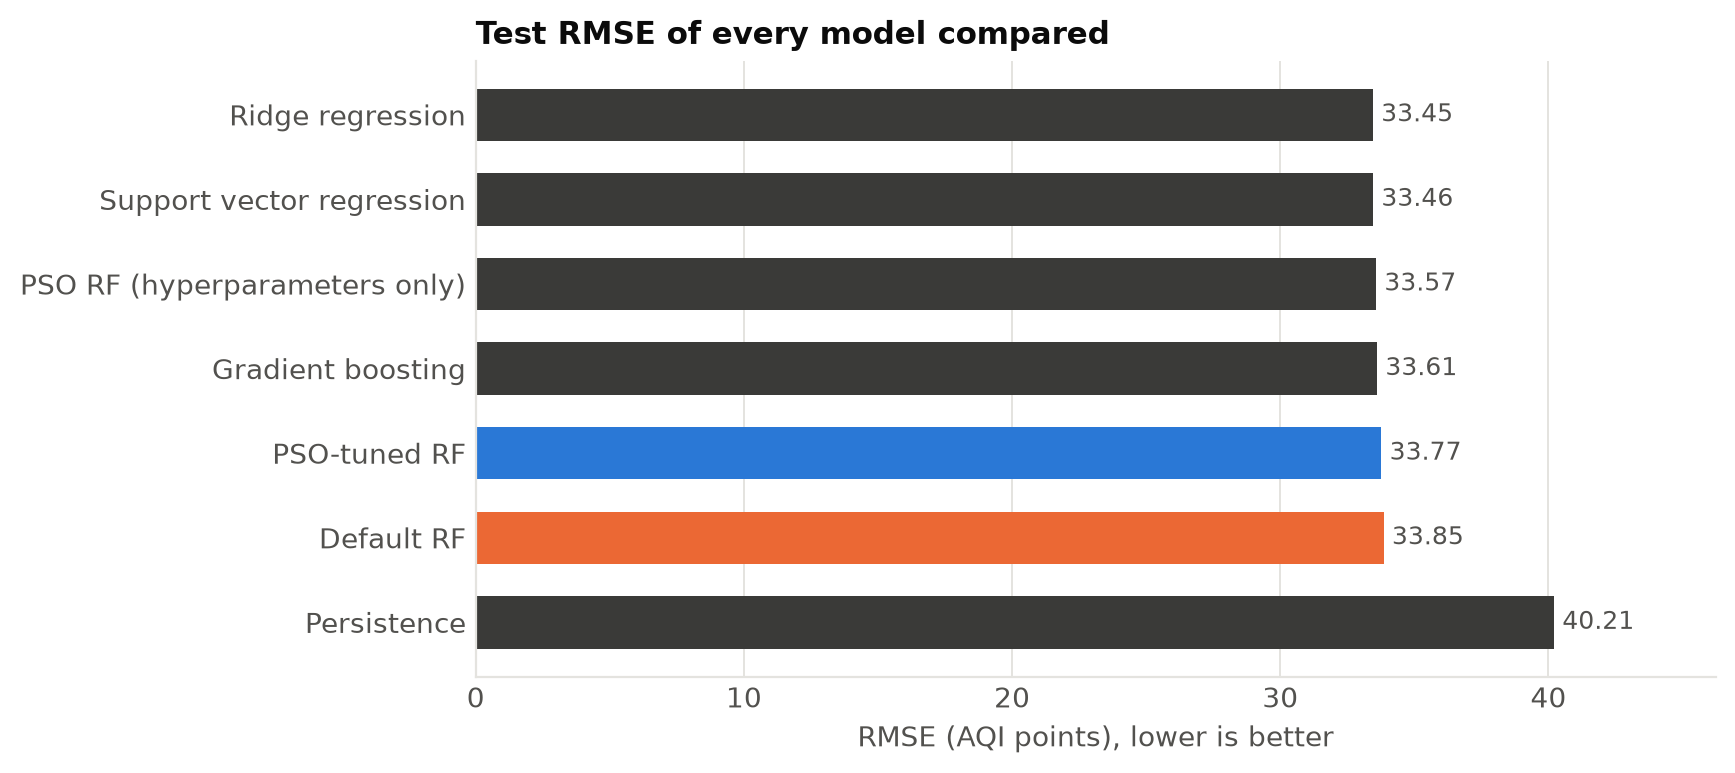
\includegraphics[width=0.82\textwidth]{figures/15_model_comparison.png}
\caption{Test RMSE of every model}
\end{figure}

\topic{PSO versus Random Search}
\begin{table}[H]
\centering
\small\setlength{\tabcolsep}{4pt}
\caption{PSO and random search with the same 312-evaluation budget (RMSE, 5 runs each)}
\begin{tabular}{|l|c|c|c|}
\hline
\textbf{Method} & \textbf{Best val.} & \textbf{Mean val.} & \textbf{Mean test} \\ \hline
Default RF & 41.52 & 41.52 & 33.81 \\
Random search, hyperparameters only & 40.75 & 40.82 & 33.62 \\
PSO, hyperparameters only & 40.66 & 40.70 & 33.55 \\
Random search, joint & 40.04 & 40.54 & 33.96 \\
\textbf{PSO, joint} & \textbf{39.73} & \textbf{39.94} & \textbf{33.47} \\ \hline
\end{tabular}
\end{table}
Test RMSE is averaged over 10 forest seeds and over the five runs of each method. In both search spaces PSO beat random search on mean validation and mean test error. The advantage is larger in the 38-dimensional joint space (0.60 validation points) than in the 6-dimensional space (0.12), because unguided sampling becomes much less effective as the number of dimensions grows. Four of the five joint PSO runs beat the best joint random-search run. Over its five runs, joint PSO also has the lowest mean test RMSE of any search (33.47, 1.0\% below the default forest).

\begin{figure}[H]
\centering
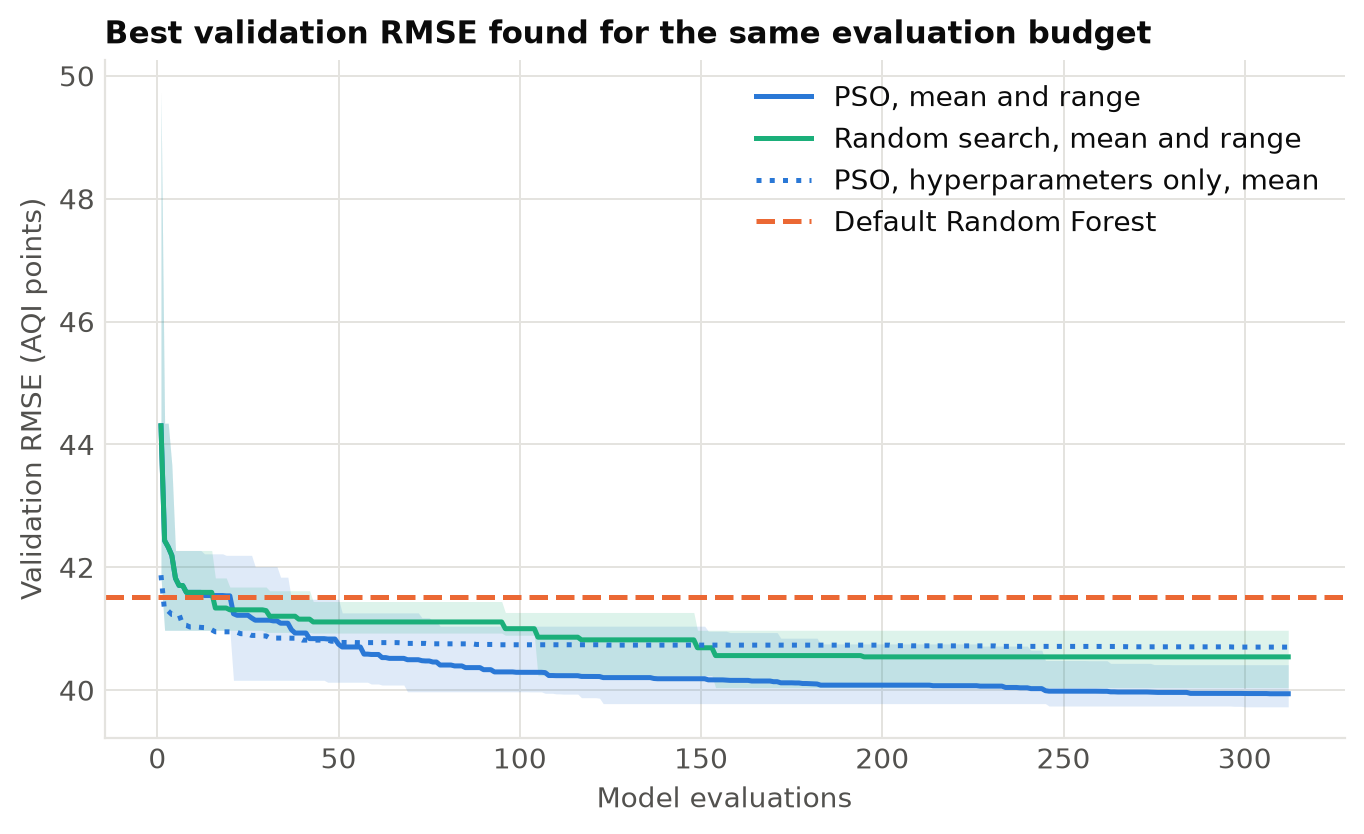
\includegraphics[width=0.88\textwidth]{figures/05_pso_vs_random_search.png}
\caption{Best validation RMSE found by PSO and random search for the same evaluation budget}
\end{figure}

\topic{Statistical Significance}
Comparison of the final PSO model with the default forest on the test period:
\begin{itemize}
\item Block-bootstrap RMSE gain: 0.09 AQI points, 95\% CI $-$0.41 to 0.59 (positive in 61.7\% of resamples)
\item Paired $t$-test on squared errors: $t = 0.31$, $p = 0.76$
\item Wilcoxon signed-rank test: $p = 0.66$
\item Final model more accurate on 49.9\% of days
\item Against persistence: gain 6.44 points, 95\% CI 4.85 to 8.06 ($p < 0.001$)
\item Against the hyperparameter-only PSO model: $-$0.20 points, 95\% CI $-$0.67 to 0.26 ($t$-test $p = 0.40$)
\end{itemize}
The improvement over persistence is highly significant. The differences between the default forest and the two PSO models are not statistically significant.

\subsection{Hyperparameter Importance Analysis}

\topic{Correlation with Performance}
Spearman correlation between each setting and validation RMSE, over all 1,560 unique configurations evaluated across the five joint PSO runs (negative means larger values lower the error):

\begin{table}[H]
\centering
\caption{Setting--fitness correlation}
\begin{tabular}{|l|c|}
\hline
\textbf{Setting} & \textbf{Spearman $\rho$ with RMSE} \\ \hline
min\_samples\_leaf & 0.659 \\
max\_depth & $-$0.346 \\
max\_samples & 0.344 \\
max\_features & $-$0.336 \\
n\_estimators & $-$0.304 \\
min\_samples\_split & 0.221 \\
Number of features used & $-$0.138 \\ \hline
\end{tabular}
\end{table}
Leaf size has the strongest effect: large leaves underfit, and the best runs used leaves of 2 to 5 days. More trees, deeper trees and more features per split all helped. The weak negative correlation for the number of features shows that the choice of \emph{which} features matters more than how many.

\subsection{Feature Importance Results}
\begin{table}[H]
\centering
\caption{Top 10 most important features of the final model (impurity-based)}
\begin{tabular}{|l|c|}
\hline
\textbf{Feature} & \textbf{Importance} \\ \hline
AQI today ($AQI_t$) & 0.635 \\
3-day mean AQI & 0.176 \\
AQI yesterday & 0.032 \\
Maximum wind speed & 0.029 \\
30-day mean AQI & 0.024 \\
Change in mean wind speed & 0.019 \\
Shortwave radiation & 0.017 \\
Rainfall & 0.016 \\
Wind direction (sine) & 0.014 \\
3-day rainfall & 0.009 \\ \hline
\end{tabular}
\end{table}
Today's AQI dominates, and AQI history accounts for 88\% of total importance. Wind, rain and radiation are the most useful weather variables: they control how quickly pollution disperses or is washed out.

\begin{figure}[H]
\centering
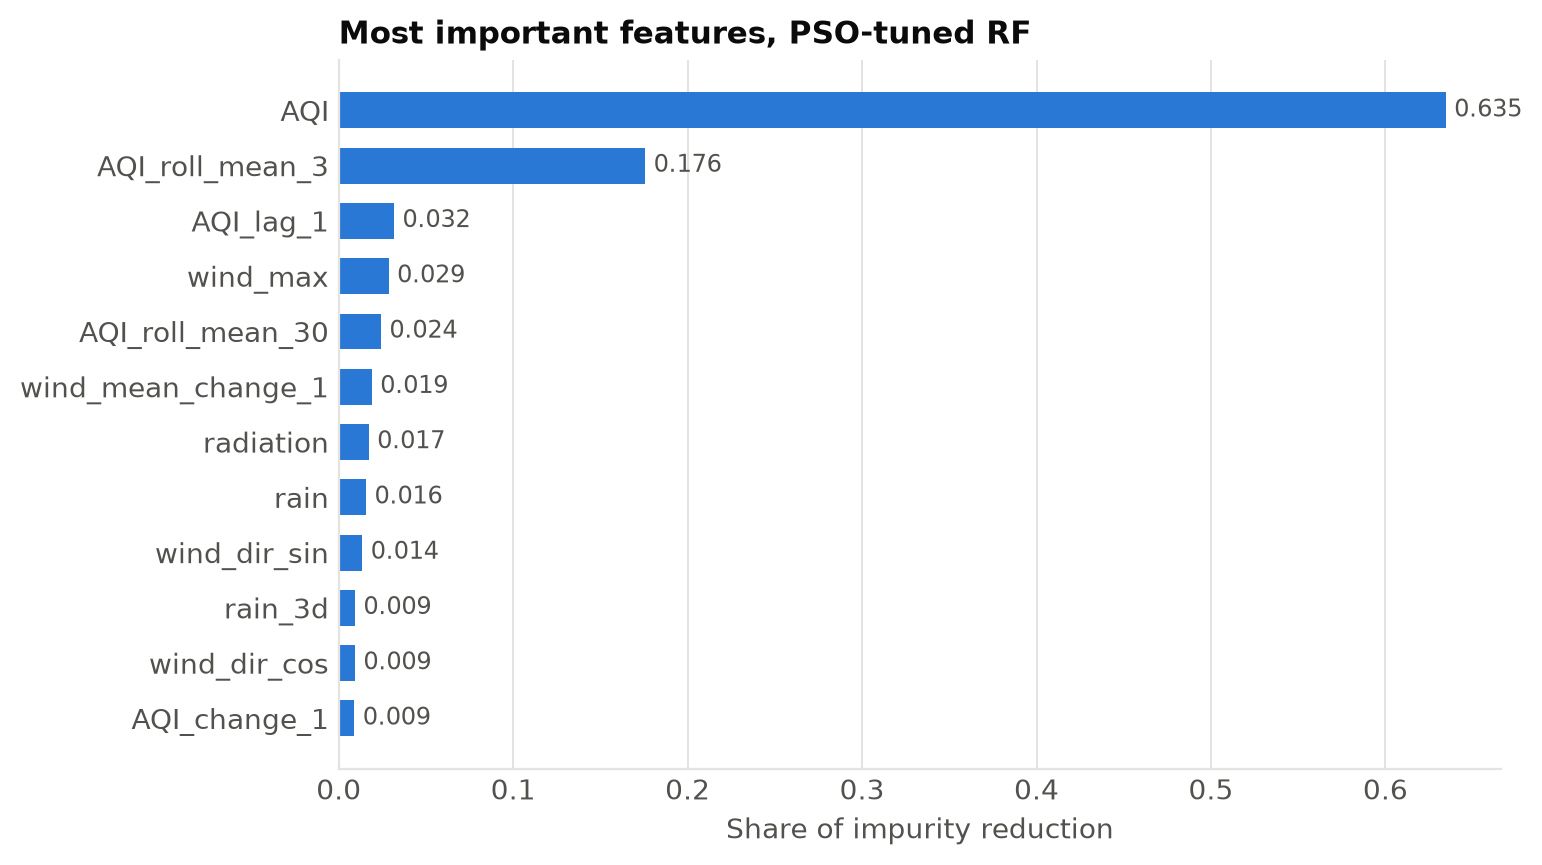
\includegraphics[width=0.75\textwidth]{figures/13_feature_importance.png}
\caption{Feature importance of the final PSO model}
\end{figure}

\subsection{Error Analysis}

\topic{Residual Distribution}
Residuals (observed minus predicted) of the final model:
\begin{itemize}
\item Mean: $-$7.72 (the model over-predicts on average)
\item Std Dev: 32.89
\item Skewness: $-$0.16 (nearly symmetric)
\item Kurtosis: 4.67 (heavier tails than a normal distribution)
\end{itemize}
Shapiro--Wilk test: $p = 1.3\times10^{-10}$, so normality is rejected because of the heavy tails.

The negative mean reflects a downward trend: the test period's mean AQI (193.8) is lower than the training period's (216.9), and the model, trained mostly on dirtier years, forecasts slightly high (mean forecast 201.5).

\begin{figure}[H]
\centering
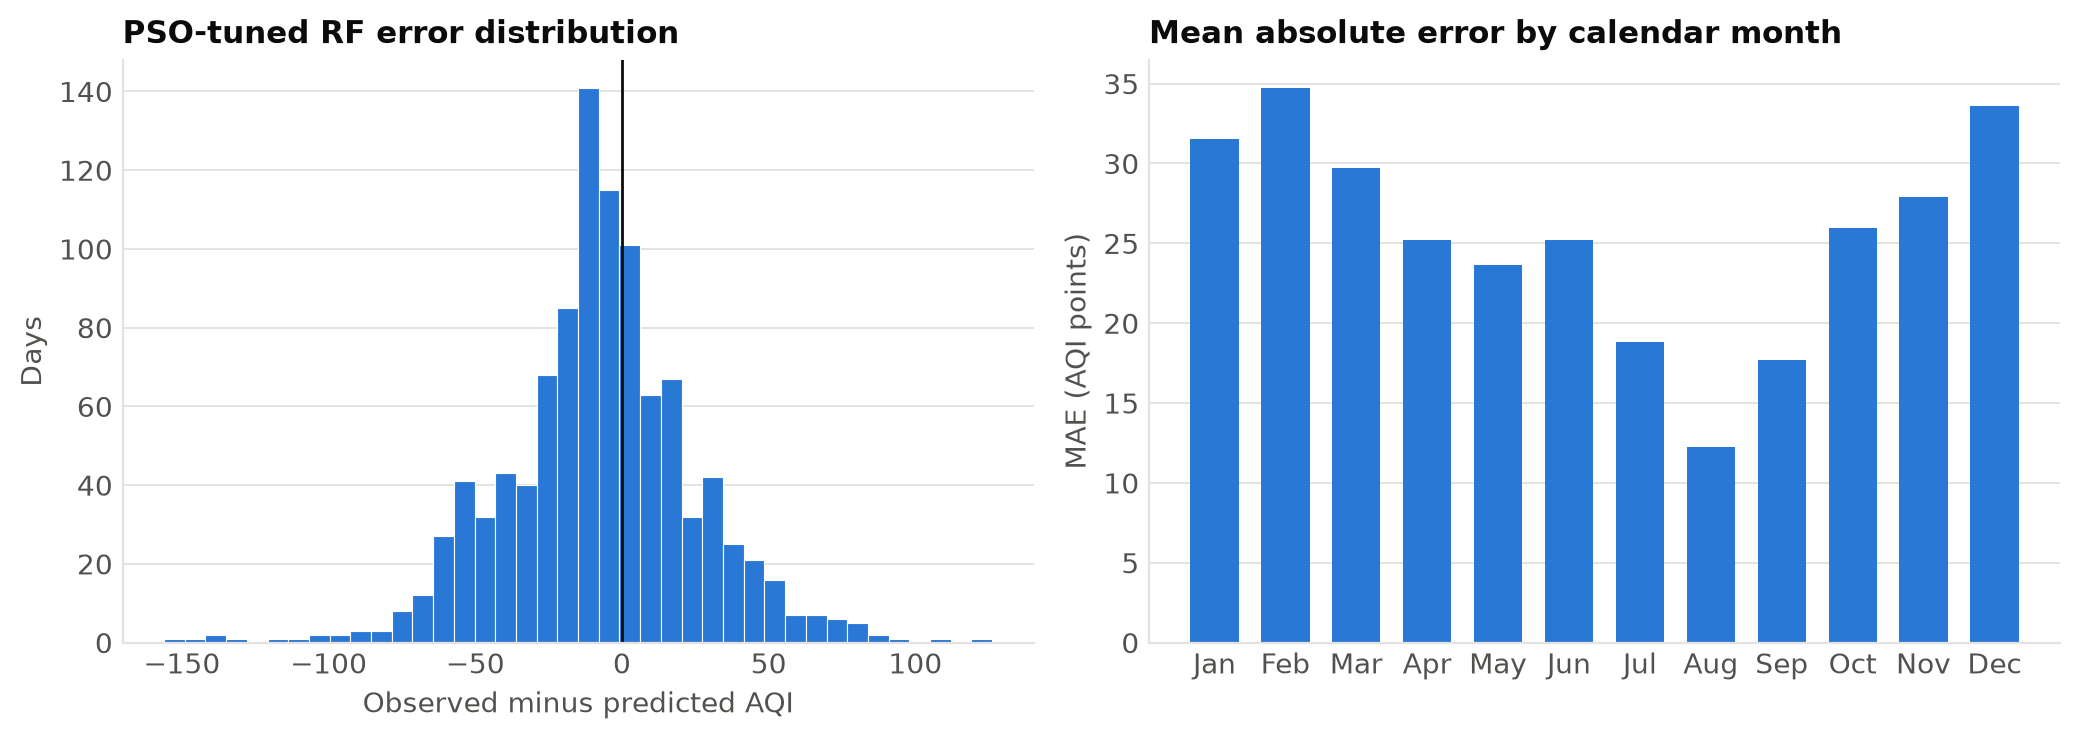
\includegraphics[width=\textwidth]{figures/11_residuals.png}
\caption{Residual distribution and mean absolute error by month}
\end{figure}

\topic{Lag on Sharp Changes}
The forecasts correlate more strongly with the previous day's AQI (0.976) than with the day being forecast (0.942), so sharp changes are followed a day late. On the 28 test days when AQI moved by more than 100 points, MAE was 87.0, against 23.4 on all other days. Such jumps are driven by events the features do not capture, such as sudden stubble-burning plumes, fireworks or a passing western disturbance.

\topic{Category Errors}
Of the 1,026 test days, 293 were placed in the wrong CPCB category, and 292 of these were only one category away. \emph{Severe} days are rare (27 days) and hard to forecast: 10 were predicted as \emph{Severe}, most of the rest as \emph{Very Poor}.

\begin{figure}[H]
\centering
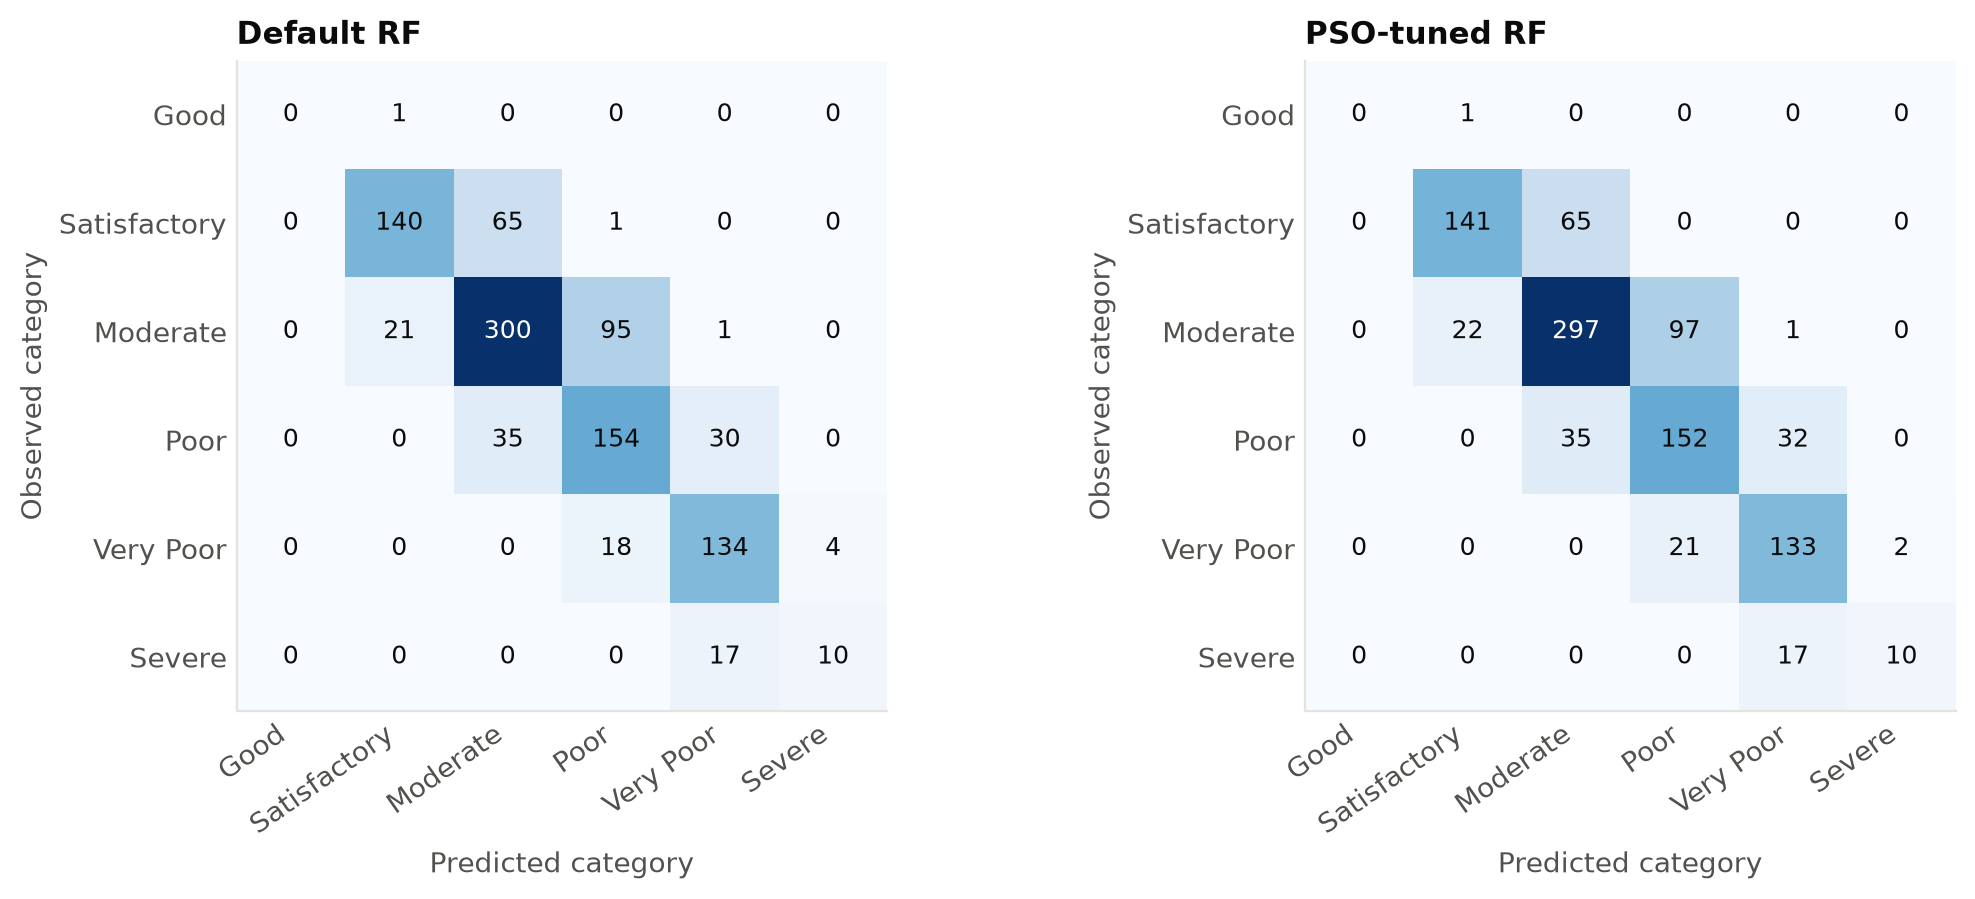
\includegraphics[width=\textwidth]{figures/14_confusion_matrices.png}
\caption{CPCB category confusion matrices on the test period}
\end{figure}

\subsection{Computational Performance}

\topic{Training Efficiency}
\begin{table}[H]
\centering
\small\setlength{\tabcolsep}{4pt}
\caption{Computational resource usage (per run)}
\begin{tabular}{|l|c|c|c|c|}
\hline
\textbf{Metric} & \textbf{PSO joint} & \textbf{RS joint} & \textbf{PSO hyp.} & \textbf{RS hyp.} \\ \hline
Fitness evaluations & 312 & 312 & 312 & 312 \\
Unique configurations trained & 312 & 312 & 307--312 & 312 \\
Forests trained per evaluation & 5 & 5 & 5 & 5 \\
Time per run (min) & 14.2--24.8 & 11.8--12.4 & 24.3--46.6 & 20.7--22.7 \\
Mean time per run (min) & 19.5 & 12.1 & 35.2 & 21.8 \\ \hline
\end{tabular}
\end{table}
The joint search is faster than the hyperparameter-only search, because each forest trains on fewer features. PSO runs take longer than random search because the swarm moves towards larger forests, which are slower to train. The search is embarrassingly parallel across runs.

\subsection{Robustness Analysis}

\topic{Stability Across Runs}
Five independent joint PSO runs with different random seeds:

\begin{table}[H]
\centering
\small
\caption{Stability across independent joint PSO runs}
\begin{tabular}{|c|c|c|c|c|c|}
\hline
\textbf{Run (seed)} & \textbf{Val. RMSE} & \textbf{Test RMSE} & \textbf{Test $R^2$} & \textbf{Features} & \textbf{Trees / depth / leaf} \\ \hline
0 (selected) & \textbf{39.73} & 33.68 & 0.882 & 14 & 224 / 18 / 2 \\
1 & 40.42 & 33.11 & 0.886 & 17 & 99 / 16 / 5 \\
2 & 39.97 & 33.53 & 0.884 & 12 & 266 / 18 / 5 \\
3 & 39.79 & 33.57 & 0.883 & 18 & 293 / 15 / 3 \\
4 & 39.81 & 33.47 & 0.884 & 18 & 187 / 22 / 3 \\ \hline
\textbf{Mean} & \textbf{39.94} & \textbf{33.47} & \textbf{0.884} & 16 & \\
\textbf{Std Dev} & \textbf{0.28} & \textbf{0.22} & \textbf{0.002} & & \\ \hline
\end{tabular}
\end{table}
Test RMSE is averaged over 10 forest seeds (the default forest averaged 33.81, SD 0.15, over the same seeds). Every joint PSO run beat the default forest on both validation and test error. However, the ranking by validation error does not carry over to the test period: the selected run (best validation) is the worst of the five on test, and run 1 (worst validation) is the best on test.

\topic{Validation Overfitting in the Larger Search}
This is the most important finding of the extension. With 38 dimensions and 312 evaluations, PSO can find feature subsets that fit the particular validation folds of 2015 to 2023 very well. Part of the 0.93-point validation gain from feature selection is therefore specific to those folds and does not transfer to 2024 to 2026. The hyperparameter-only search, with only 6 dimensions, has less freedom to overfit its validation folds: the standard deviation of its five test RMSEs is only 0.04 points, against 0.22 for the joint search. Remedies include a longer or more recent validation window, penalizing the number of features in the fitness, or averaging the forests found by several runs.

\topic{Learning Curves}
With a fixed validation window (the last 20\% of the training period), the gap between training and validation RMSE at full size is 21.1 points for the default forest (15.1 vs 36.2), 11.2 points for the hyperparameter-only PSO forest (24.8 vs 36.0) and 9.2 points for the final model (27.3 vs 36.5). PSO's regularization more than halved the overfitting gap of individual trees.

\begin{figure}[H]
\centering
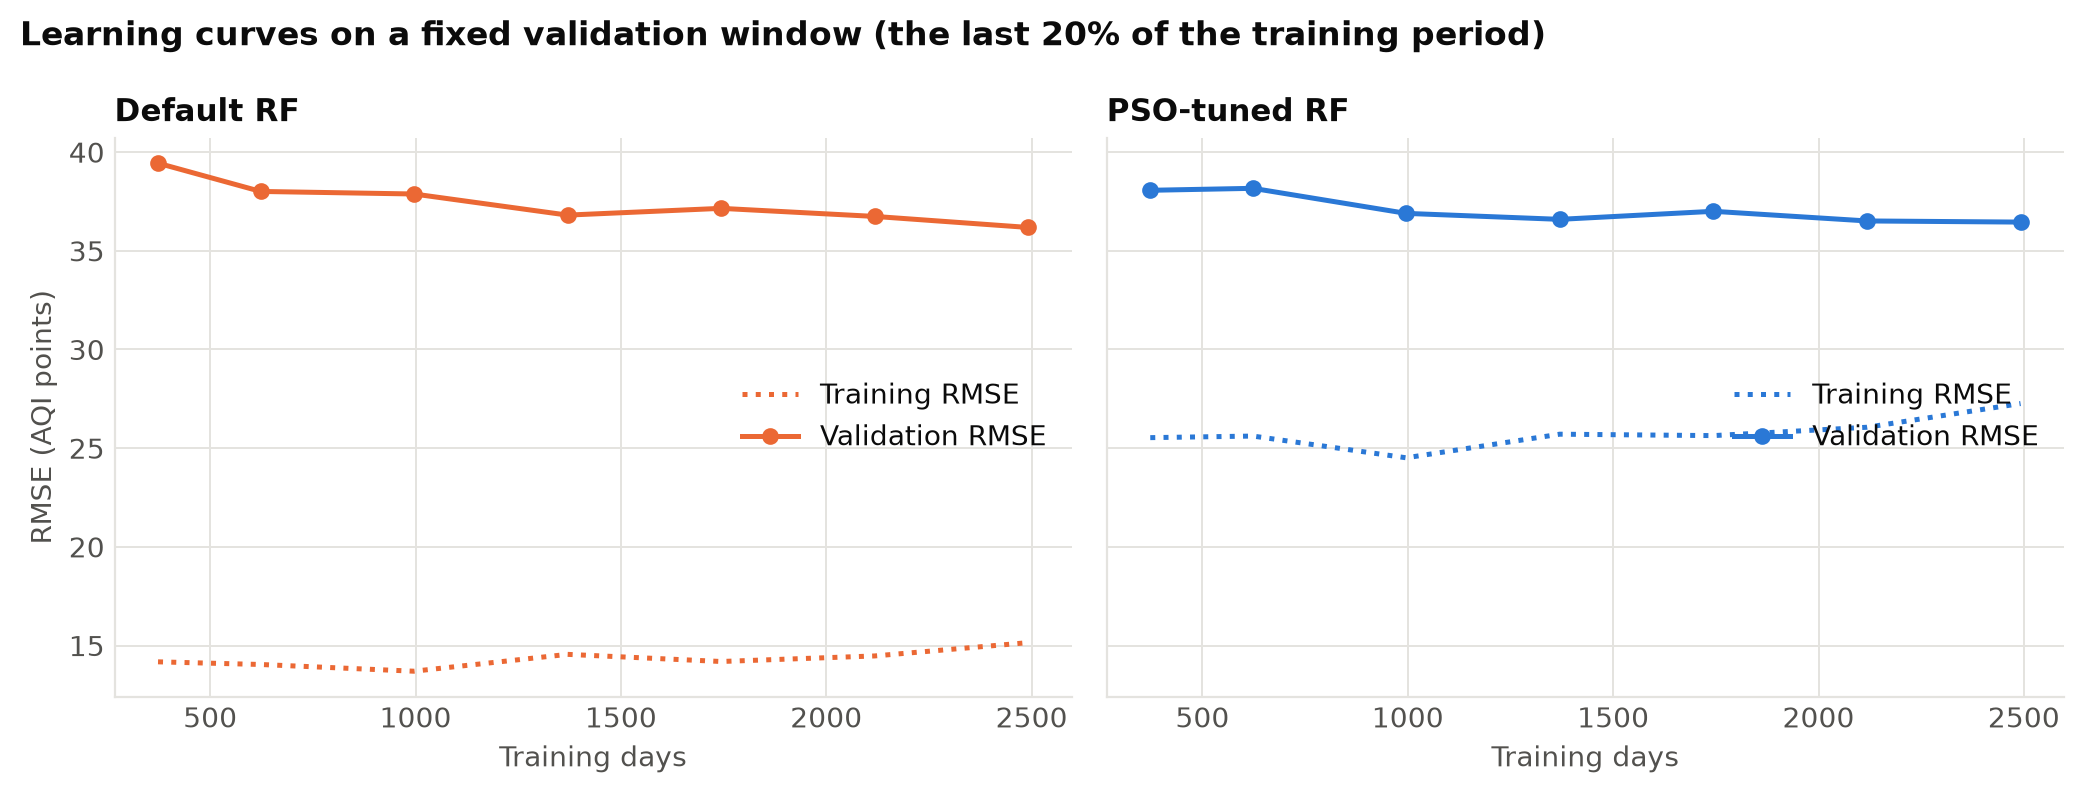
\includegraphics[width=\textwidth]{figures/12_learning_curves.png}
\caption{Learning curves of the default and final PSO Random Forest}
\end{figure}

\subsection{Discussion}

\topic{Why PSO Works Here}
Several factors contribute:
\begin{enumerate}
\item \textbf{Guided search:} Sharing the global best moves particles quickly to good regions, which is why PSO beat random search in both search spaces, and by more in the larger one
\item \textbf{No gradient dependence:} The noisy, stepped validation error and the binary feature switches are handled naturally
\item \textbf{Exploration then exploitation:} Decreasing inertia gave a broad early search and a focused late search, visible in the diversity curve
\item \textbf{Physically sensible selection:} PSO kept wind, rain and radiation and discarded redundant humidity, pressure and lag features without being told which variables matter
\end{enumerate}

\topic{Why the Test Gain over the Default Is Small}
\begin{itemize}
\item Random Forest defaults are already strong on tabular data, so there is little error left for tuning to remove
\item AQI history carries most of the predictive signal (88\% of total importance), and every model uses it
\item The largest gain came from features and model choice: moving from persistence to any learned model cut RMSE by 6 to 7 points; tuning changed it by 0.1 to 0.3
\item In the joint search, part of the validation gain was overfitting to the validation folds
\end{itemize}

\topic{Limitations}
\begin{itemize}
\item \textbf{Not statistically significant:} Neither PSO model is significantly better than the default forest on the test period
\item \textbf{Validation overfitting:} The selected joint model was 2.3\% better on validation than the hyperparameter-only model but 0.6\% worse on test
\item \textbf{Linear models competitive:} Ridge regression matched the forests, so the forest's complexity is not essential here
\item \textbf{Reactive forecasts:} Sharp jumps are followed a day late
\item \textbf{Observed, not forecast, weather:} The model uses today's weather; tomorrow's forecast weather could add information but is not in the archive used
\item \textbf{Single city:} Results apply to Delhi
\end{itemize}

\topic{Practical Implications}
\begin{itemize}
\item The model forecasts next-day AQI within about 25 AQI points on average, and flags \emph{Very Poor} days with AUC 0.986
\item It needs only 14 inputs instead of 32, which simplifies data collection for deployment
\item Retraining each year is advisable, given the downward trend in Delhi's AQI
\end{itemize}

\begin{figure}[H]
\centering
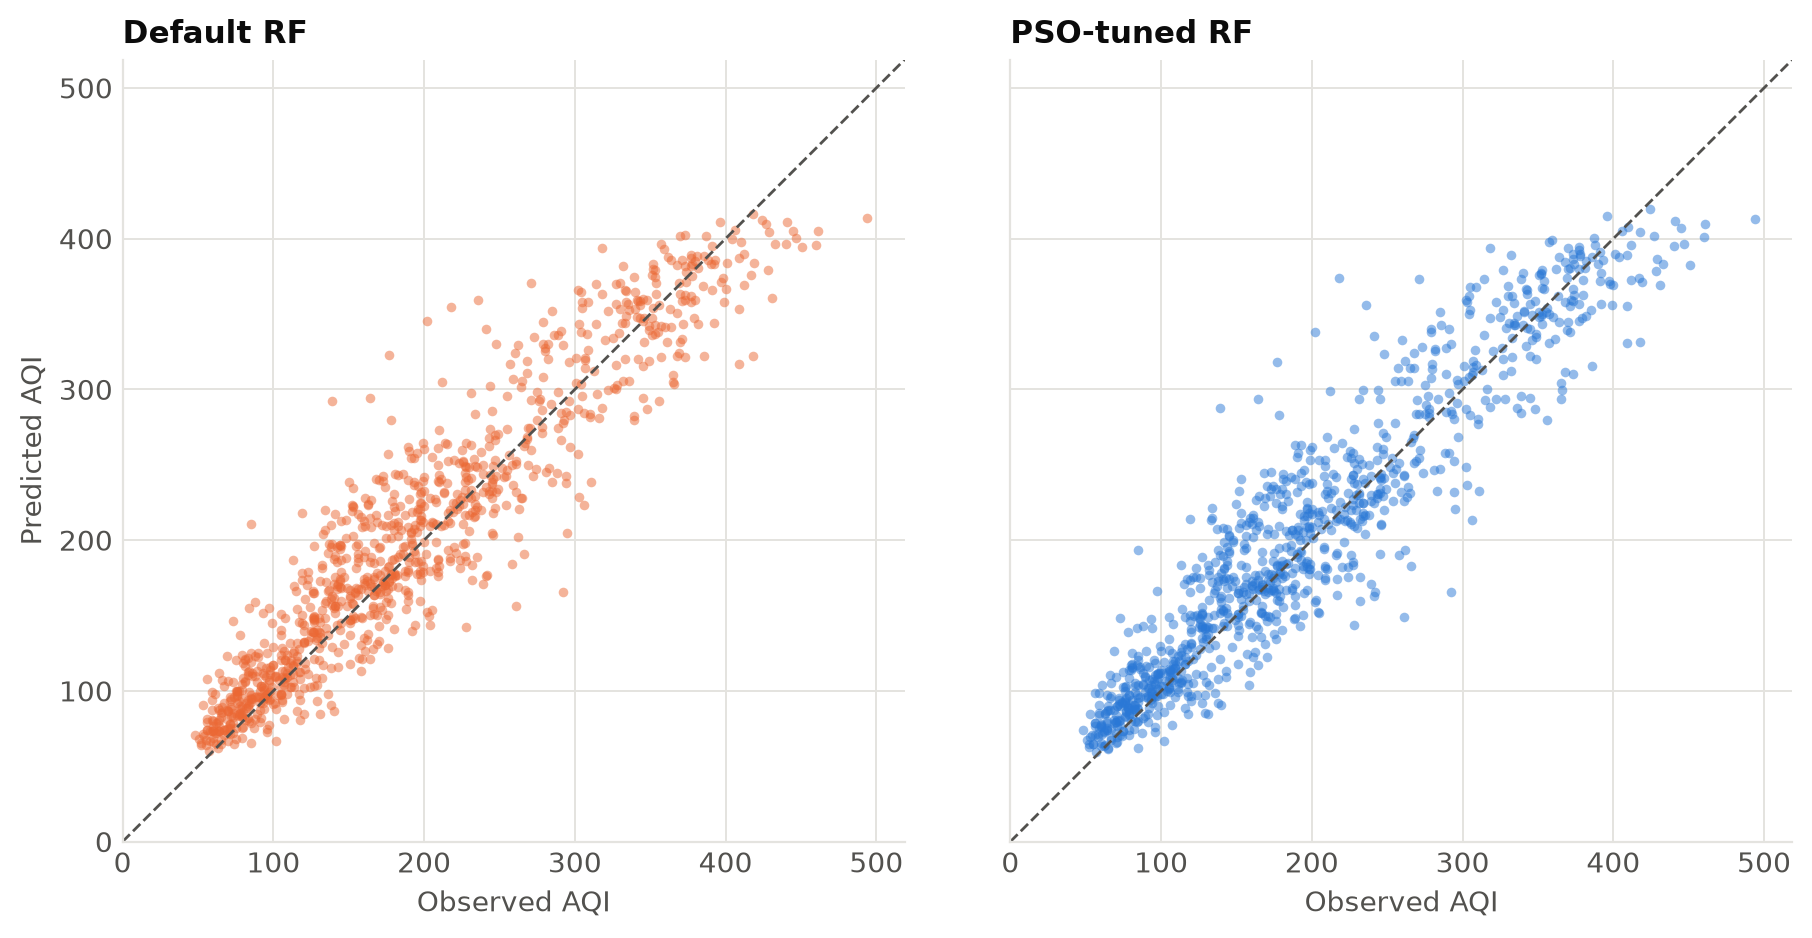
\includegraphics[width=\textwidth]{figures/10_actual_vs_predicted.png}
\caption{Model performance before optimization (left, default RF) and after PSO optimization (right)}
\end{figure}

%================================================================ 0.8
\section{Conclusion}
This project built and evaluated a Random Forest optimized by Particle Swarm Optimization for next-day AQI forecasting in Delhi, using 4,170 days of official CPCB bulletins and ERA5 weather from 2015 to 2026. PSO was implemented from first principles and verified on benchmark functions, where it solved the Sphere function to machine precision.

PSO searched the six Random Forest hyperparameters and the choice of input features together, in a 38-dimensional space with threshold-based feature switches. It reduced walk-forward validation RMSE by 4.3\% (41.52 to 39.73), twice the 2.1\% reached by tuning hyperparameters alone, and it beat random search with the same budget in both search spaces, by a wider margin in the larger one. It kept 14 of 32 features, consistently choosing wind, rain and radiation and discarding redundant humidity, pressure and lag variables.

On the held-out 2024--2026 period, the selected model achieved an RMSE of 33.77 and an $R^2$ of 0.882, 16.0\% better than persistence. Averaged over its five runs, joint PSO gave the lowest test RMSE of any search (33.47, 1.0\% below the default forest). However, the selected model's gain over the default forest was small (0.25\%) and not statistically significant, and it was slightly worse than the hyperparameter-only model, showing that the larger search partly overfitted its validation folds. PSO is an effective optimizer for this task, but for next-day AQI forecasting, good features and weather inputs matter more than tuning, and a larger search space must be paired with a more robust validation scheme.

%================================================================ 0.9
\section{Future Work}
While this project establishes a solid foundation, several directions remain for future investigation:

\subsection{Methodological Enhancements}

\topic{Better Inputs}
\textbf{Forecast Weather:} Use tomorrow's numerical weather forecast instead of today's observed weather, so the model can anticipate changes in wind and rain rather than react to them.

\textbf{Fire and Emission Data:} Add satellite fire counts from Punjab and Haryana and festival calendars, which drive the sharp autumn jumps the model currently misses.

\textbf{Multi-City Data:} Train one model across several Indo-Gangetic cities to learn shared regional patterns.

\topic{Improved Optimization Strategies}
\textbf{More Robust Fitness:} Penalize the number of features, use a more recent validation window, or evaluate each particle on several forest seeds, so the joint search overfits its validation folds less.

\textbf{Ensembles of Runs:} Average the forests found by several PSO runs; the five-run mean test RMSE (33.47) suggests this would be more reliable than picking one run.

\textbf{Other Nature-Inspired Optimizers:} Compare PSO with Genetic Algorithms, Differential Evolution and Grey Wolf Optimizer on the same budget and fitness function.

\textbf{Weighted Fitness:} Optimize an error that weights \emph{Very Poor} and \emph{Severe} days more heavily, since those forecasts matter most for public health.

\textbf{Surrogate-Assisted PSO:} Use a cheap surrogate model of the fitness to reduce the cost of each search.

\topic{Model Extensions}
\textbf{Gradient Boosting and Deep Models:} Apply the same PSO framework to gradient boosting and to sequence models such as LSTMs, which have more hyperparameters and may gain more from tuning.

\textbf{Probabilistic Forecasts:} Provide prediction intervals, so that alerts can be issued with a stated level of confidence.

\clearpage
\renewcommand{\bibname}{References}
\begingroup
\renewcommand{\chapter}[2]{\section*{#2}\addcontentsline{toc}{section}{References}}
\begin{thebibliography}{99}
\setlength{\itemsep}{2pt}
\bibitem{kennedy1995} J. Kennedy and R. Eberhart, ``Particle swarm optimization,'' in \emph{Proc. IEEE International Conference on Neural Networks (ICNN'95)}, vol.~4, pp.~1942--1948, 1995.
\bibitem{shi1998} Y. Shi and R. Eberhart, ``A modified particle swarm optimizer,'' in \emph{Proc. IEEE International Conference on Evolutionary Computation}, pp.~69--73, 1998.
\bibitem{clerc2002} M. Clerc and J. Kennedy, ``The particle swarm: explosion, stability, and convergence in a multidimensional complex space,'' \emph{IEEE Transactions on Evolutionary Computation}, vol.~6, no.~1, pp.~58--73, 2002.
\bibitem{breiman2001} L. Breiman, ``Random forests,'' \emph{Machine Learning}, vol.~45, no.~1, pp.~5--32, 2001.
\bibitem{probst2019} P. Probst, M. N. Wright and A.-L. Boulesteix, ``Hyperparameters and tuning strategies for random forest,'' \emph{WIREs Data Mining and Knowledge Discovery}, vol.~9, no.~3, e1301, 2019.
\bibitem{bergstra2012} J. Bergstra and Y. Bengio, ``Random search for hyper-parameter optimization,'' \emph{Journal of Machine Learning Research}, vol.~13, pp.~281--305, 2012.
\bibitem{snoek2012} J. Snoek, H. Larochelle and R. P. Adams, ``Practical Bayesian optimization of machine learning algorithms,'' in \emph{Advances in Neural Information Processing Systems 25}, 2012.
\bibitem{boxjenkins} G. E. P. Box and G. M. Jenkins, \emph{Time Series Analysis: Forecasting and Control}. San Francisco: Holden-Day, 1970.
\bibitem{hochreiter1997} S. Hochreiter and J. Schmidhuber, ``Long short-term memory,'' \emph{Neural Computation}, vol.~9, no.~8, pp.~1735--1780, 1997.
\bibitem{holland1975} J. H. Holland, \emph{Adaptation in Natural and Artificial Systems}. Ann Arbor: University of Michigan Press, 1975.
\bibitem{dorigo1996} M. Dorigo, V. Maniezzo and A. Colorni, ``Ant system: optimization by a colony of cooperating agents,'' \emph{IEEE Transactions on Systems, Man, and Cybernetics, Part B}, vol.~26, no.~1, pp.~29--41, 1996.
\bibitem{kirkpatrick1983} S. Kirkpatrick, C. D. Gelatt and M. P. Vecchi, ``Optimization by simulated annealing,'' \emph{Science}, vol.~220, no.~4598, pp.~671--680, 1983.
\bibitem{storn1997} R. Storn and K. Price, ``Differential evolution: a simple and efficient heuristic for global optimization over continuous spaces,'' \emph{Journal of Global Optimization}, vol.~11, no.~4, pp.~341--359, 1997.
\bibitem{wolpert1997} D. H. Wolpert and W. G. Macready, ``No free lunch theorems for optimization,'' \emph{IEEE Transactions on Evolutionary Computation}, vol.~1, no.~1, pp.~67--82, 1997.
\bibitem{kunsch1989} H. R. K\"unsch, ``The jackknife and the bootstrap for general stationary observations,'' \emph{The Annals of Statistics}, vol.~17, no.~3, pp.~1217--1241, 1989.
\bibitem{guttikunda2012} S. K. Guttikunda and B. R. Gurjar, ``Role of meteorology in seasonality of air pollution in megacity Delhi, India,'' \emph{Environmental Monitoring and Assessment}, vol.~184, no.~5, pp.~3199--3211, 2012.
\bibitem{cpcb2014} Central Pollution Control Board, \emph{National Air Quality Index}, Control of Urban Pollution Series CUPS/82/2014-15. New Delhi: CPCB, 2014.
\bibitem{hersbach2020} H. Hersbach \emph{et al.}, ``The ERA5 global reanalysis,'' \emph{Quarterly Journal of the Royal Meteorological Society}, vol.~146, no.~730, pp.~1999--2049, 2020.
\bibitem{urbanemissions} UrbanEmissions.info, ``AQI\_bulletins: daily AQI bulletins from CPCB for Indian cities,'' GitHub repository, \url{https://github.com/urbanemissions-info/AQI_bulletins}, accessed 6 November 2026.
\bibitem{openmeteo} Open-Meteo, ``Historical Weather API,'' \url{https://open-meteo.com/en/docs/historical-weather-api}, accessed 6 November 2026.
\end{thebibliography}
\endgroup



\end{document}
